% =============================================================================
% main.tex — root file, only assembles the parts. Build: see README.md (the skill's compile_latex.sh)
% =============================================================================
\documentclass[11pt,a4paper]{article}
% =============================================================================
% preamble.tex — packages and settings shared by the report
% Engine: pdflatex. English, single column.
% =============================================================================

% --- Harmless warning filters (load before the packages that emit them) -------
\usepackage{silence}
\WarningFilter{microtype}{I cannot find a protrusion list}

% --- Encoding and fonts -------------------------------------------------------
\usepackage[utf8]{inputenc}
\usepackage[T1]{fontenc}
\usepackage{lmodern}
\usepackage[english]{babel}

% --- Page layout --------------------------------------------------------------
\usepackage[a4paper, margin=2.5cm, headheight=13.6pt]{geometry} % headheight as fancyhdr requires at 12pt
\usepackage{microtype}
\usepackage{setspace}
\setstretch{1.05}
\usepackage{fancyhdr}
\pagestyle{fancy}
\fancyhf{}
\fancyhead[L]{\small\nouppercase{\FirstMark{2e-left}}} % first section on the page (\leftmark gives the last)
\fancyfoot[C]{\small\thepage}
\renewcommand{\headrulewidth}{0.4pt}

% Float placement: allow fuller text pages with floats, fewer float-only pages
\renewcommand{\topfraction}{0.85}
\renewcommand{\bottomfraction}{0.6}
\renewcommand{\textfraction}{0.12}
\renewcommand{\floatpagefraction}{0.75}
\setcounter{topnumber}{3}
\setcounter{totalnumber}{4}

% No widows or orphans (long-form best practices)
\widowpenalty=10000
\clubpenalty=10000

% --- Mathematics --------------------------------------------------------------
\usepackage{mathtools}            % loads amsmath
\usepackage{amssymb}
\usepackage{amsthm}
\usepackage{bm}

\theoremstyle{plain}
\newtheorem{theorem}{Theorem}[section]
\newtheorem{lemma}[theorem]{Lemma}
\newtheorem{proposition}[theorem]{Proposition}
\newtheorem{corollary}[theorem]{Corollary}
\theoremstyle{definition}
\newtheorem{definition}[theorem]{Definition}
\newtheorem{example}[theorem]{Example}
\theoremstyle{remark}
\newtheorem{remark}[theorem]{Remark}

% Frequent math commands
\newcommand{\R}{\mathbb{R}}
\newcommand{\N}{\mathbb{N}}
\newcommand{\E}{\mathbb{E}}
\newcommand{\Prob}{\mathbb{P}}
\newcommand{\ind}{\mathbf{1}}
\DeclareMathOperator*{\argmax}{arg\,max}
\DeclareMathOperator*{\argmin}{arg\,min}
\DeclarePairedDelimiter{\abs}{\lvert}{\rvert}
\DeclarePairedDelimiter{\norm}{\lVert}{\rVert}
\DeclarePairedDelimiter{\set}{\{}{\}}

% --- Figures and tables -------------------------------------------------------
\usepackage{graphicx}
\graphicspath{{figures/}}
\usepackage[font=small,labelfont=bf,labelsep=period,format=hang]{caption}
\usepackage{subcaption}
\usepackage{booktabs}
\usepackage{array}
\usepackage{multirow}
\usepackage{tabularx}
\usepackage{longtable}
\usepackage{float}
\usepackage[table]{xcolor}
\usepackage{csvsimple}           % tables read directly from CSV (skill: Tables from CSV Data)
\usepackage{pgfplots}             % plots from CSV (skill: charts-and-graphs)
\pgfplotsset{compat=1.18}
\usepgfplotslibrary{groupplots}  % sensitivity grid
\usepackage{fontawesome5}          % icons for the system-model scene
\definecolor{groundgreen}{RGB}{168,196,116}
\usetikzlibrary{arrows.meta, positioning, calc, fit, backgrounds, shapes.geometric, shapes.misc, decorations.pathmorphing}

% --- Lists (compact spacing) --------------------------------------------------
\usepackage{enumitem}
\setlist[itemize]{nosep, leftmargin=*, topsep=2pt, partopsep=0pt}
\setlist[enumerate]{nosep, leftmargin=*, topsep=2pt, partopsep=0pt}

% --- Pseudocode ---------------------------------------------------------------
\usepackage{algorithm}
\usepackage{algpseudocode}
\algrenewcommand\algorithmicrequire{\textbf{Input:}}
\algrenewcommand\algorithmicensure{\textbf{Output:}}

% --- Units and numbers --------------------------------------------------------
\usepackage{siunitx}
\sisetup{detect-all, per-mode=symbol}  % units as kbit/s
\DeclareSIUnit{\dBm}{dBm}         % siunitx has no dBm
\DeclareSIUnit{\dB}{dB}

% --- Bibliography -------------------------------------------------------------
\usepackage{csquotes}
\usepackage[backend=biber, style=ieee, sorting=none, maxbibnames=6]{biblatex}
\AtBeginBibliography{\small\raggedright}  % long hyphenated titles do not break; ragged right keeps them in the margin
% \addbibresource lives in main.tex so that the skill's compile_latex.sh detects biber

% --- Links and cross-references (load late) -----------------------------------
\usepackage[unicode, colorlinks=true, linkcolor=blue!60!black,
            citecolor=blue!60!black, urlcolor=blue!60!black]{hyperref}
\usepackage[nameinlink]{cleveref}
\crefname{equation}{Eq.}{Eqs.}
\Crefname{equation}{Equation}{Equations}
\crefname{appendix}{Appendix}{Appendices}
\crefname{subsection}{Section}{Sections}
\crefname{section}{Section}{Sections}
\crefname{figure}{Figure}{Figures}
\crefname{table}{Table}{Tables}
\crefname{algorithm}{Algorithm}{Algorithms}
\crefname{proposition}{Proposition}{Propositions}
\crefname{definition}{Definition}{Definitions}
\crefname{remark}{Remark}{Remarks}

% Generated by experiments/report_tables.py from results/phase1; do not edit.
\newcommand{\ResultTimelyVzeroBzero}{\num{0.413}}
\newcommand{\ResultTimelyLowVzeroBzero}{\num{0.319}}
\newcommand{\ResultTimelyHighVzeroBzero}{\num{0.487}}
\newcommand{\ResultConnVzeroBzero}{\num{0.509}}
\newcommand{\ResultBoundVzeroBzero}{\num{0.483}}
\newcommand{\ResultGapVzeroBzero}{\num{0.171}}
\newcommand{\ResultPlanningVzeroBzero}{\num{0.000}}
\newcommand{\ResultEvaluationVzeroBzero}{\num{0.040}}
\newcommand{\ResultBoundTimeVzeroBzero}{\num{0.494}}
\newcommand{\ResultGapUndefinedVzeroBzero}{0}
\newcommand{\ResultTimelyVzeroBone}{\num{0.494}}
\newcommand{\ResultTimelyLowVzeroBone}{\num{0.391}}
\newcommand{\ResultTimelyHighVzeroBone}{\num{0.582}}
\newcommand{\ResultConnVzeroBone}{\num{1.000}}
\newcommand{\ResultBoundVzeroBone}{\num{0.621}}
\newcommand{\ResultGapVzeroBone}{\num{0.238}}
\newcommand{\ResultPlanningVzeroBone}{\num{0.210}}
\newcommand{\ResultEvaluationVzeroBone}{\num{0.043}}
\newcommand{\ResultBoundTimeVzeroBone}{\num{2.987}}
\newcommand{\ResultGapUndefinedVzeroBone}{0}
\newcommand{\ResultTimelyVzeroBhfivezeroBzero}{\num{0.370}}
\newcommand{\ResultTimelyLowVzeroBhfivezeroBzero}{\num{0.283}}
\newcommand{\ResultTimelyHighVzeroBhfivezeroBzero}{\num{0.437}}
\newcommand{\ResultConnVzeroBhfivezeroBzero}{\num{0.509}}
\newcommand{\ResultBoundVzeroBhfivezeroBzero}{\num{0.468}}
\newcommand{\ResultGapVzeroBhfivezeroBzero}{\num{0.229}}
\newcommand{\ResultPlanningVzeroBhfivezeroBzero}{\num{0.000}}
\newcommand{\ResultEvaluationVzeroBhfivezeroBzero}{\num{0.036}}
\newcommand{\ResultBoundTimeVzeroBhfivezeroBzero}{\num{1.719}}
\newcommand{\ResultGapUndefinedVzeroBhfivezeroBzero}{0}
\newcommand{\ResultTimelyVzeroBhfivezeroBone}{\num{0.430}}
\newcommand{\ResultTimelyLowVzeroBhfivezeroBone}{\num{0.344}}
\newcommand{\ResultTimelyHighVzeroBhfivezeroBone}{\num{0.500}}
\newcommand{\ResultConnVzeroBhfivezeroBone}{\num{1.000}}
\newcommand{\ResultBoundVzeroBhfivezeroBone}{\num{0.585}}
\newcommand{\ResultGapVzeroBhfivezeroBone}{\num{0.287}}
\newcommand{\ResultPlanningVzeroBhfivezeroBone}{\num{0.197}}
\newcommand{\ResultEvaluationVzeroBhfivezeroBone}{\num{0.035}}
\newcommand{\ResultBoundTimeVzeroBhfivezeroBone}{\num{6.898}}
\newcommand{\ResultGapUndefinedVzeroBhfivezeroBone}{0}
\newcommand{\ResultLpCount}{3600}
\newcommand{\ResultLpRuntimeMedian}{\num{1.85}}
\newcommand{\ResultLpRuntimeMax}{\num{44.4}}
\newcommand{\ResultLpVariablesMedian}{23203}
\newcommand{\ResultLpVariablesMax}{74062}
\newcommand{\ResultMilpCount}{5}
\newcommand{\ResultMilpOptimalCount}{5}
\newcommand{\ResultTangentOverestimateMax}{\num{0.0242}}
\newcommand{\ResultComputeMinutes}{\num{184}}
\newcommand{\ResultMilpMethodAtOptimumCount}{4}
\newcommand{\ResultMilpStaticTotal}{4}
\newcommand{\ResultMilpEqualSplitTotal}{20}
\newcommand{\ResultMilpPlanAtOptimumCount}{4}
\newcommand{\ResultWorkers}{12}
\newcommand{\ResultCpuCount}{12}
\newcommand{\ResultScenarioCount}{30}
\newcommand{\ResultPythonVersion}{3.12.3}
\newcommand{\ResultScipyVersion}{1.18.1}
\newcommand{\ResultHighsVersion}{1.12.0}
\newcommand{\ResultBoneWinsVzero}{26}
\newcommand{\ResultBoneTiesVzero}{3}
\newcommand{\ResultBoneWinsVzeroBhfivezero}{27}
\newcommand{\ResultBoneTiesVzeroBhfivezero}{0}
  % baseline (B0, B1, bound, MILP) result macros, written by experiments/report_tables.py
% Generated by experiments/report_tables_phase2.py from results/phase2; do not edit.
\newcommand{\ResultTwoTimelyVzeroBzero}{\num{0.413}}
\newcommand{\ResultTwoTimelyLowVzeroBzero}{\num{0.319}}
\newcommand{\ResultTwoTimelyHighVzeroBzero}{\num{0.487}}
\newcommand{\ResultTwoConnVzeroBzero}{\num{0.509}}
\newcommand{\ResultTwoGapVzeroBzero}{\num{0.171}}
\newcommand{\ResultTwoUnionGapVzeroBzero}{\num{0.428}}
\newcommand{\ResultTwoUnionBoundVzeroBzero}{\num{0.678}}
\newcommand{\ResultTwoPlanningVzeroBzero}{\num{0.0}}
\newcommand{\ResultTwoCallsVzeroBzero}{\num{1}}
\newcommand{\ResultTwoOutsideVzeroBzero}{\num{0.0}}
\newcommand{\ResultTwoTimelyVzeroBone}{\num{0.494}}
\newcommand{\ResultTwoTimelyLowVzeroBone}{\num{0.391}}
\newcommand{\ResultTwoTimelyHighVzeroBone}{\num{0.582}}
\newcommand{\ResultTwoConnVzeroBone}{\num{1.000}}
\newcommand{\ResultTwoGapVzeroBone}{\num{0.238}}
\newcommand{\ResultTwoUnionGapVzeroBone}{\num{0.305}}
\newcommand{\ResultTwoUnionBoundVzeroBone}{\num{0.678}}
\newcommand{\ResultTwoPlanningVzeroBone}{\num{0.2}}
\newcommand{\ResultTwoCallsVzeroBone}{\num{1}}
\newcommand{\ResultTwoOutsideVzeroBone}{\num{0.0}}
\newcommand{\ResultTwoTimelyVzeroBtwo}{\num{0.559}}
\newcommand{\ResultTwoTimelyLowVzeroBtwo}{\num{0.452}}
\newcommand{\ResultTwoTimelyHighVzeroBtwo}{\num{0.648}}
\newcommand{\ResultTwoConnVzeroBtwo}{\num{1.000}}
\newcommand{\ResultTwoGapVzeroBtwo}{\num{0.191}}
\newcommand{\ResultTwoUnionGapVzeroBtwo}{\num{0.204}}
\newcommand{\ResultTwoUnionBoundVzeroBtwo}{\num{0.678}}
\newcommand{\ResultTwoPlanningVzeroBtwo}{\num{172.3}}
\newcommand{\ResultTwoCallsVzeroBtwo}{\num{1861}}
\newcommand{\ResultTwoOutsideVzeroBtwo}{\num{5.7}}
\newcommand{\ResultTwoTimelyVzeroBthree}{\num{0.369}}
\newcommand{\ResultTwoTimelyLowVzeroBthree}{\num{0.283}}
\newcommand{\ResultTwoTimelyHighVzeroBthree}{\num{0.445}}
\newcommand{\ResultTwoConnVzeroBthree}{\num{1.000}}
\newcommand{\ResultTwoGapVzeroBthree}{\num{0.471}}
\newcommand{\ResultTwoUnionGapVzeroBthree}{\num{0.492}}
\newcommand{\ResultTwoUnionBoundVzeroBthree}{\num{0.678}}
\newcommand{\ResultTwoPlanningVzeroBthree}{\num{206.8}}
\newcommand{\ResultTwoCallsVzeroBthree}{\num{1950}}
\newcommand{\ResultTwoOutsideVzeroBthree}{\num{11.8}}
\newcommand{\ResultTwoTimelyVzeroP}{\num{0.560}}
\newcommand{\ResultTwoTimelyLowVzeroP}{\num{0.448}}
\newcommand{\ResultTwoTimelyHighVzeroP}{\num{0.656}}
\newcommand{\ResultTwoConnVzeroP}{\num{1.000}}
\newcommand{\ResultTwoGapVzeroP}{\num{0.190}}
\newcommand{\ResultTwoUnionGapVzeroP}{\num{0.205}}
\newcommand{\ResultTwoUnionBoundVzeroP}{\num{0.678}}
\newcommand{\ResultTwoPlanningVzeroP}{\num{181.1}}
\newcommand{\ResultTwoCallsVzeroP}{\num{1975}}
\newcommand{\ResultTwoOutsideVzeroP}{\num{5.3}}
\newcommand{\ResultTwoHigherVzeroBtwoBzero}{30}
\newcommand{\ResultTwoEqualVzeroBtwoBzero}{0}
\newcommand{\ResultTwoLowerVzeroBtwoBzero}{0}
\newcommand{\ResultTwoHigherVzeroBtwoBone}{29}
\newcommand{\ResultTwoEqualVzeroBtwoBone}{0}
\newcommand{\ResultTwoLowerVzeroBtwoBone}{1}
\newcommand{\ResultTwoHigherVzeroPBtwo}{16}
\newcommand{\ResultTwoEqualVzeroPBtwo}{4}
\newcommand{\ResultTwoLowerVzeroPBtwo}{10}
\newcommand{\ResultTwoHigherVzeroBoneBzero}{26}
\newcommand{\ResultTwoEqualVzeroBoneBzero}{3}
\newcommand{\ResultTwoLowerVzeroBoneBzero}{1}
\newcommand{\ResultTwoTimelyVzeroBhfivezeroBzero}{\num{0.370}}
\newcommand{\ResultTwoTimelyLowVzeroBhfivezeroBzero}{\num{0.283}}
\newcommand{\ResultTwoTimelyHighVzeroBhfivezeroBzero}{\num{0.437}}
\newcommand{\ResultTwoConnVzeroBhfivezeroBzero}{\num{0.509}}
\newcommand{\ResultTwoGapVzeroBhfivezeroBzero}{\num{0.229}}
\newcommand{\ResultTwoUnionGapVzeroBhfivezeroBzero}{\num{0.450}}
\newcommand{\ResultTwoUnionBoundVzeroBhfivezeroBzero}{\num{0.636}}
\newcommand{\ResultTwoPlanningVzeroBhfivezeroBzero}{\num{0.0}}
\newcommand{\ResultTwoCallsVzeroBhfivezeroBzero}{\num{1}}
\newcommand{\ResultTwoOutsideVzeroBhfivezeroBzero}{\num{0.0}}
\newcommand{\ResultTwoTimelyVzeroBhfivezeroBone}{\num{0.430}}
\newcommand{\ResultTwoTimelyLowVzeroBhfivezeroBone}{\num{0.344}}
\newcommand{\ResultTwoTimelyHighVzeroBhfivezeroBone}{\num{0.500}}
\newcommand{\ResultTwoConnVzeroBhfivezeroBone}{\num{1.000}}
\newcommand{\ResultTwoGapVzeroBhfivezeroBone}{\num{0.287}}
\newcommand{\ResultTwoUnionGapVzeroBhfivezeroBone}{\num{0.350}}
\newcommand{\ResultTwoUnionBoundVzeroBhfivezeroBone}{\num{0.636}}
\newcommand{\ResultTwoPlanningVzeroBhfivezeroBone}{\num{0.2}}
\newcommand{\ResultTwoCallsVzeroBhfivezeroBone}{\num{1}}
\newcommand{\ResultTwoOutsideVzeroBhfivezeroBone}{\num{0.0}}
\newcommand{\ResultTwoTimelyVzeroBhfivezeroBtwo}{\num{0.517}}
\newcommand{\ResultTwoTimelyLowVzeroBhfivezeroBtwo}{\num{0.423}}
\newcommand{\ResultTwoTimelyHighVzeroBhfivezeroBtwo}{\num{0.598}}
\newcommand{\ResultTwoConnVzeroBhfivezeroBtwo}{\num{1.000}}
\newcommand{\ResultTwoGapVzeroBhfivezeroBtwo}{\num{0.199}}
\newcommand{\ResultTwoUnionGapVzeroBhfivezeroBtwo}{\num{0.213}}
\newcommand{\ResultTwoUnionBoundVzeroBhfivezeroBtwo}{\num{0.636}}
\newcommand{\ResultTwoPlanningVzeroBhfivezeroBtwo}{\num{212.6}}
\newcommand{\ResultTwoCallsVzeroBhfivezeroBtwo}{\num{1941}}
\newcommand{\ResultTwoOutsideVzeroBhfivezeroBtwo}{\num{7.7}}
\newcommand{\ResultTwoTimelyVzeroBhfivezeroBthree}{\num{0.336}}
\newcommand{\ResultTwoTimelyLowVzeroBhfivezeroBthree}{\num{0.260}}
\newcommand{\ResultTwoTimelyHighVzeroBhfivezeroBthree}{\num{0.402}}
\newcommand{\ResultTwoConnVzeroBhfivezeroBthree}{\num{1.000}}
\newcommand{\ResultTwoGapVzeroBhfivezeroBthree}{\num{0.484}}
\newcommand{\ResultTwoUnionGapVzeroBhfivezeroBthree}{\num{0.503}}
\newcommand{\ResultTwoUnionBoundVzeroBhfivezeroBthree}{\num{0.636}}
\newcommand{\ResultTwoPlanningVzeroBhfivezeroBthree}{\num{248.4}}
\newcommand{\ResultTwoCallsVzeroBhfivezeroBthree}{\num{1969}}
\newcommand{\ResultTwoOutsideVzeroBhfivezeroBthree}{\num{14.0}}
\newcommand{\ResultTwoTimelyVzeroBhfivezeroP}{\num{0.521}}
\newcommand{\ResultTwoTimelyLowVzeroBhfivezeroP}{\num{0.425}}
\newcommand{\ResultTwoTimelyHighVzeroBhfivezeroP}{\num{0.601}}
\newcommand{\ResultTwoConnVzeroBhfivezeroP}{\num{1.000}}
\newcommand{\ResultTwoGapVzeroBhfivezeroP}{\num{0.191}}
\newcommand{\ResultTwoUnionGapVzeroBhfivezeroP}{\num{0.204}}
\newcommand{\ResultTwoUnionBoundVzeroBhfivezeroP}{\num{0.636}}
\newcommand{\ResultTwoPlanningVzeroBhfivezeroP}{\num{214.8}}
\newcommand{\ResultTwoCallsVzeroBhfivezeroP}{\num{2001}}
\newcommand{\ResultTwoOutsideVzeroBhfivezeroP}{\num{8.4}}
\newcommand{\ResultTwoHigherVzeroBhfivezeroBtwoBzero}{30}
\newcommand{\ResultTwoEqualVzeroBhfivezeroBtwoBzero}{0}
\newcommand{\ResultTwoLowerVzeroBhfivezeroBtwoBzero}{0}
\newcommand{\ResultTwoHigherVzeroBhfivezeroBtwoBone}{30}
\newcommand{\ResultTwoEqualVzeroBhfivezeroBtwoBone}{0}
\newcommand{\ResultTwoLowerVzeroBhfivezeroBtwoBone}{0}
\newcommand{\ResultTwoHigherVzeroBhfivezeroPBtwo}{17}
\newcommand{\ResultTwoEqualVzeroBhfivezeroPBtwo}{1}
\newcommand{\ResultTwoLowerVzeroBhfivezeroPBtwo}{12}
\newcommand{\ResultTwoHigherVzeroBhfivezeroBoneBzero}{27}
\newcommand{\ResultTwoEqualVzeroBhfivezeroBoneBzero}{0}
\newcommand{\ResultTwoLowerVzeroBhfivezeroBoneBzero}{3}
\newcommand{\ResultTwoScenarioCount}{30}
\newcommand{\ResultTwoDiffVzeroPBtwo}{\num{0.002}}
\newcommand{\ResultTwoDiffLowVzeroPBtwo}{\num{-0.008}}
\newcommand{\ResultTwoDiffHighVzeroPBtwo}{\num{0.015}}
\newcommand{\ResultTwoHolmVzeroPBtwo}{\num{0.8477}}
\newcommand{\ResultTwoRankBiserialVzeroPBtwo}{\num{0.02}}
\newcommand{\ResultTwoDiffVzeroBtwoBone}{\num{0.064}}
\newcommand{\ResultTwoDiffLowVzeroBtwoBone}{\num{0.044}}
\newcommand{\ResultTwoDiffHighVzeroBtwoBone}{\num{0.086}}
\newcommand{\ResultTwoHolmVzeroBtwoBone}{\num{0.0156}}
\newcommand{\ResultTwoRankBiserialVzeroBtwoBone}{\num{1.00}}
\newcommand{\ResultTwoDiffVzeroBtwoBthree}{\num{0.190}}
\newcommand{\ResultTwoDiffLowVzeroBtwoBthree}{\num{0.157}}
\newcommand{\ResultTwoDiffHighVzeroBtwoBthree}{\num{0.226}}
\newcommand{\ResultTwoHolmVzeroBtwoBthree}{\num{0.0156}}
\newcommand{\ResultTwoRankBiserialVzeroBtwoBthree}{\num{1.00}}
\newcommand{\ResultTwoDiffVzeroPBone}{\num{0.066}}
\newcommand{\ResultTwoDiffLowVzeroPBone}{\num{0.046}}
\newcommand{\ResultTwoDiffHighVzeroPBone}{\num{0.088}}
\newcommand{\ResultTwoHolmVzeroPBone}{\num{0.0156}}
\newcommand{\ResultTwoRankBiserialVzeroPBone}{\num{1.00}}
\newcommand{\ResultTwoDiffVzeroBhfivezeroPBtwo}{\num{0.003}}
\newcommand{\ResultTwoDiffLowVzeroBhfivezeroPBtwo}{\num{-0.004}}
\newcommand{\ResultTwoDiffHighVzeroBhfivezeroPBtwo}{\num{0.010}}
\newcommand{\ResultTwoHolmVzeroBhfivezeroPBtwo}{\num{0.7969}}
\newcommand{\ResultTwoRankBiserialVzeroBhfivezeroPBtwo}{\num{0.31}}
\newcommand{\ResultTwoDiffVzeroBhfivezeroBtwoBone}{\num{0.087}}
\newcommand{\ResultTwoDiffLowVzeroBhfivezeroBtwoBone}{\num{0.065}}
\newcommand{\ResultTwoDiffHighVzeroBhfivezeroBtwoBone}{\num{0.112}}
\newcommand{\ResultTwoHolmVzeroBhfivezeroBtwoBone}{\num{0.0156}}
\newcommand{\ResultTwoRankBiserialVzeroBhfivezeroBtwoBone}{\num{1.00}}
\newcommand{\ResultTwoDiffVzeroBhfivezeroBtwoBthree}{\num{0.181}}
\newcommand{\ResultTwoDiffLowVzeroBhfivezeroBtwoBthree}{\num{0.145}}
\newcommand{\ResultTwoDiffHighVzeroBhfivezeroBtwoBthree}{\num{0.220}}
\newcommand{\ResultTwoHolmVzeroBhfivezeroBtwoBthree}{\num{0.0156}}
\newcommand{\ResultTwoRankBiserialVzeroBhfivezeroBtwoBthree}{\num{1.00}}
\newcommand{\ResultTwoDiffVzeroBhfivezeroPBone}{\num{0.091}}
\newcommand{\ResultTwoDiffLowVzeroBhfivezeroPBone}{\num{0.070}}
\newcommand{\ResultTwoDiffHighVzeroBhfivezeroPBone}{\num{0.112}}
\newcommand{\ResultTwoHolmVzeroBhfivezeroPBone}{\num{0.0156}}
\newcommand{\ResultTwoRankBiserialVzeroBhfivezeroPBone}{\num{1.00}}
\newcommand{\ResultTwoHolmFloor}{\num{0.0156}}
\newcommand{\ResultTwoAblationDiffVzeroPOpone}{\num{-0.001}}
\newcommand{\ResultTwoAblationTimelyVzeroPOpone}{\num{0.560}}
\newcommand{\ResultTwoAblationDiffVzeroBhfivezeroPOpone}{\num{-0.005}}
\newcommand{\ResultTwoAblationTimelyVzeroBhfivezeroPOpone}{\num{0.516}}
\newcommand{\ResultTwoAblationDiffVzeroPOptwo}{\num{0.001}}
\newcommand{\ResultTwoAblationTimelyVzeroPOptwo}{\num{0.562}}
\newcommand{\ResultTwoAblationDiffVzeroBhfivezeroPOptwo}{\num{0.001}}
\newcommand{\ResultTwoAblationTimelyVzeroBhfivezeroPOptwo}{\num{0.521}}
\newcommand{\ResultTwoAblationDiffVzeroPNoBacklog}{\num{-0.002}}
\newcommand{\ResultTwoAblationTimelyVzeroPNoBacklog}{\num{0.558}}
\newcommand{\ResultTwoAblationDiffVzeroBhfivezeroPNoBacklog}{\num{0.001}}
\newcommand{\ResultTwoAblationTimelyVzeroBhfivezeroPNoBacklog}{\num{0.522}}
\newcommand{\ResultTwoAblationDiffVzeroPFixedPaths}{\num{-0.045}}
\newcommand{\ResultTwoAblationTimelyVzeroPFixedPaths}{\num{0.515}}
\newcommand{\ResultTwoAblationDiffVzeroBhfivezeroPFixedPaths}{\num{-0.068}}
\newcommand{\ResultTwoAblationTimelyVzeroBhfivezeroPFixedPaths}{\num{0.453}}
\newcommand{\ResultTwoAblationDiffVzeroPFixedTrajectory}{\num{-0.041}}
\newcommand{\ResultTwoAblationTimelyVzeroPFixedTrajectory}{\num{0.519}}
\newcommand{\ResultTwoAblationDiffVzeroBhfivezeroPFixedTrajectory}{\num{-0.032}}
\newcommand{\ResultTwoAblationTimelyVzeroBhfivezeroPFixedTrajectory}{\num{0.489}}
\newcommand{\ResultTwoAblationDiffVzeroPEqualBandwidth}{\num{0.003}}
\newcommand{\ResultTwoAblationTimelyVzeroPEqualBandwidth}{\num{0.564}}
\newcommand{\ResultTwoAblationDiffVzeroBhfivezeroPEqualBandwidth}{\num{-0.003}}
\newcommand{\ResultTwoAblationTimelyVzeroBhfivezeroPEqualBandwidth}{\num{0.518}}
\newcommand{\ResultTwoAblationDiffVzeroPExpectedDesign}{\num{-0.038}}
\newcommand{\ResultTwoAblationTimelyVzeroPExpectedDesign}{\num{0.523}}
\newcommand{\ResultTwoAblationDiffVzeroBhfivezeroPExpectedDesign}{\num{-0.045}}
\newcommand{\ResultTwoAblationTimelyVzeroBhfivezeroPExpectedDesign}{\num{0.476}}
\newcommand{\ResultTwoAblationDiffVzeroPCatalogTrajectory}{\num{0.006}}
\newcommand{\ResultTwoAblationTimelyVzeroPCatalogTrajectory}{\num{0.567}}
\newcommand{\ResultTwoAblationDiffVzeroBhfivezeroPCatalogTrajectory}{\num{0.008}}
\newcommand{\ResultTwoAblationTimelyVzeroBhfivezeroPCatalogTrajectory}{\num{0.528}}
\newcommand{\ResultTwoTercileGainVzeroLow}{\num{0.104}}
\newcommand{\ResultTwoTercileGainVzeroMiddle}{\num{0.162}}
\newcommand{\ResultTwoTercileGainVzeroHigh}{\num{0.170}}
\newcommand{\ResultTwoGroundCorrelationVzero}{\num{0.90}}
\newcommand{\ResultTwoTercileGainVzeroBhfivezeroLow}{\num{0.118}}
\newcommand{\ResultTwoTercileGainVzeroBhfivezeroMiddle}{\num{0.144}}
\newcommand{\ResultTwoTercileGainVzeroBhfivezeroHigh}{\num{0.184}}
\newcommand{\ResultTwoGroundCorrelationVzeroBhfivezero}{\num{0.87}}
\newcommand{\ResultTwoBudgetBtwoTwofivezero}{\num{0.513}}
\newcommand{\ResultTwoBudgetCallsBtwoTwofivezero}{\num{251}}
\newcommand{\ResultTwoBudgetBtwoFivezerozero}{\num{0.530}}
\newcommand{\ResultTwoBudgetCallsBtwoFivezerozero}{\num{501}}
\newcommand{\ResultTwoBudgetBtwoOnezerozerozero}{\num{0.547}}
\newcommand{\ResultTwoBudgetCallsBtwoOnezerozerozero}{\num{990}}
\newcommand{\ResultTwoBudgetBtwoTwozerozerozero}{\num{0.559}}
\newcommand{\ResultTwoBudgetCallsBtwoTwozerozerozero}{\num{1861}}
\newcommand{\ResultTwoBudgetBtwoFourzerozerozero}{\num{0.560}}
\newcommand{\ResultTwoBudgetCallsBtwoFourzerozerozero}{\num{1897}}
\newcommand{\ResultTwoBudgetPTwofivezero}{\num{0.518}}
\newcommand{\ResultTwoBudgetCallsPTwofivezero}{\num{251}}
\newcommand{\ResultTwoBudgetPFivezerozero}{\num{0.532}}
\newcommand{\ResultTwoBudgetCallsPFivezerozero}{\num{501}}
\newcommand{\ResultTwoBudgetPOnezerozerozero}{\num{0.546}}
\newcommand{\ResultTwoBudgetCallsPOnezerozerozero}{\num{1001}}
\newcommand{\ResultTwoBudgetPTwozerozerozero}{\num{0.560}}
\newcommand{\ResultTwoBudgetCallsPTwozerozerozero}{\num{1975}}
\newcommand{\ResultTwoBudgetPFourzerozerozero}{\num{0.562}}
\newcommand{\ResultTwoBudgetCallsPFourzerozerozero}{\num{2261}}
\newcommand{\ResultTwoSensSensAlertstwozeroBone}{\num{0.462}}
\newcommand{\ResultTwoSensSensAlertstwozeroBtwo}{\num{0.529}}
\newcommand{\ResultTwoSensSensAlertstwozeroP}{\num{0.543}}
\newcommand{\ResultTwoSensSensAlertssixzeroBone}{\num{0.440}}
\newcommand{\ResultTwoSensSensAlertssixzeroBtwo}{\num{0.499}}
\newcommand{\ResultTwoSensSensAlertssixzeroP}{\num{0.498}}
\newcommand{\ResultTwoSensSensBhonezerozeroBone}{\num{0.430}}
\newcommand{\ResultTwoSensSensBhonezerozeroBtwo}{\num{0.521}}
\newcommand{\ResultTwoSensSensBhonezerozeroP}{\num{0.511}}
\newcommand{\ResultTwoSensSensBtotzerofiveBone}{\num{0.446}}
\newcommand{\ResultTwoSensSensBtotzerofiveBtwo}{\num{0.523}}
\newcommand{\ResultTwoSensSensBtotzerofiveP}{\num{0.532}}
\newcommand{\ResultTwoSensSensBtottwoBone}{\num{0.461}}
\newcommand{\ResultTwoSensSensBtottwoBtwo}{\num{0.546}}
\newcommand{\ResultTwoSensSensBtottwoP}{\num{0.534}}
\newcommand{\ResultTwoSensSensDeadlineLongBone}{\num{0.485}}
\newcommand{\ResultTwoSensSensDeadlineLongBtwo}{\num{0.637}}
\newcommand{\ResultTwoSensSensDeadlineLongP}{\num{0.635}}
\newcommand{\ResultTwoSensSensDeadlineShortBone}{\num{0.367}}
\newcommand{\ResultTwoSensSensDeadlineShortBtwo}{\num{0.392}}
\newcommand{\ResultTwoSensSensDeadlineShortP}{\num{0.388}}
\newcommand{\ResultTwoSensSensKtwoBone}{\num{0.451}}
\newcommand{\ResultTwoSensSensKtwoBtwo}{\num{0.516}}
\newcommand{\ResultTwoSensSensKtwoP}{\num{0.514}}
\newcommand{\ResultTwoSensSensKfiveBone}{\num{0.458}}
\newcommand{\ResultTwoSensSensKfiveBtwo}{\num{0.515}}
\newcommand{\ResultTwoSensSensKfiveP}{\num{0.517}}
\newcommand{\ResultTwoSensSensLrefonetwofivekBone}{\num{0.536}}
\newcommand{\ResultTwoSensSensLrefonetwofivekBtwo}{\num{0.599}}
\newcommand{\ResultTwoSensSensLrefonetwofivekP}{\num{0.590}}
\newcommand{\ResultTwoSensSensLrefonemBone}{\num{0.274}}
\newcommand{\ResultTwoSensSensLrefonemBtwo}{\num{0.340}}
\newcommand{\ResultTwoSensSensLrefonemP}{\num{0.311}}
\newcommand{\ResultTwoSensSensLreffivezerozerokBone}{\num{0.363}}
\newcommand{\ResultTwoSensSensLreffivezerozerokBtwo}{\num{0.416}}
\newcommand{\ResultTwoSensSensLreffivezerozerokP}{\num{0.417}}
\newcommand{\ResultTwoSensSensPhysicalBone}{\num{1.000}}
\newcommand{\ResultTwoSensSensPhysicalBtwo}{\num{1.000}}
\newcommand{\ResultTwoSensSensPhysicalP}{\num{1.000}}
\newcommand{\ResultTwoSensVzeroBone}{\num{0.455}}
\newcommand{\ResultTwoSensVzeroBtwo}{\num{0.535}}
\newcommand{\ResultTwoSensVzeroP}{\num{0.529}}
\newcommand{\ResultTwoSensVzeroBhfivezeroBone}{\num{0.389}}
\newcommand{\ResultTwoSensVzeroBhfivezeroBtwo}{\num{0.487}}
\newcommand{\ResultTwoSensVzeroBhfivezeroP}{\num{0.489}}
\newcommand{\ResultTwoDesignExpected}{\num{0.492}}
\newcommand{\ResultTwoDesignPlanningExpected}{\num{34.1}}
\newcommand{\ResultTwoDesignOne}{\num{0.488}}
\newcommand{\ResultTwoDesignPlanningOne}{\num{35.4}}
\newcommand{\ResultTwoDesignFive}{\num{0.529}}
\newcommand{\ResultTwoDesignPlanningFive}{\num{211.6}}
\newcommand{\ResultTwoDesignOnezero}{\num{0.524}}
\newcommand{\ResultTwoDesignPlanningOnezero}{\num{262.7}}
\newcommand{\ResultTwoLpCount}{13500}
\newcommand{\ResultTwoLpOptimalCount}{13500}
\newcommand{\ResultTwoComputeHours}{\num{71.9}}
\newcommand{\ResultTwoSensitivityScenarioCount}{10}
  % result macros of the proposed methods, written by experiments/report_tables_phase2.py
% Generated by experiments/report_tables_extensions.py from results/phase1, results/phase2 and data/manifests; do not edit.
\newcommand{\ResultExtTimelyVzeroBone}{\num{0.494}}
\newcommand{\ResultExtGapVzeroBone}{\num{0.238}}
\newcommand{\ResultExtPlanningVzeroBone}{\num{0.2}}
\newcommand{\ResultExtConnVzeroBone}{\num{1.000}}
\newcommand{\ResultExtTimelyVzeroBtwo}{\num{0.559}}
\newcommand{\ResultExtGapVzeroBtwo}{\num{0.191}}
\newcommand{\ResultExtPlanningVzeroBtwo}{\num{172.3}}
\newcommand{\ResultExtConnVzeroBtwo}{\num{1.000}}
\newcommand{\ResultExtTimelyVzeroP}{\num{0.560}}
\newcommand{\ResultExtGapVzeroP}{\num{0.190}}
\newcommand{\ResultExtPlanningVzeroP}{\num{181.1}}
\newcommand{\ResultExtConnVzeroP}{\num{1.000}}
\newcommand{\ResultExtTimelyVzeroTRAN}{\num{0.530}}
\newcommand{\ResultExtGapVzeroTRAN}{\num{0.304}}
\newcommand{\ResultExtPlanningVzeroTRAN}{\num{234.2}}
\newcommand{\ResultExtConnVzeroTRAN}{\num{0.999}}
\newcommand{\ResultExtTimelyVzeroBhfivezeroBone}{\num{0.430}}
\newcommand{\ResultExtGapVzeroBhfivezeroBone}{\num{0.287}}
\newcommand{\ResultExtPlanningVzeroBhfivezeroBone}{\num{0.2}}
\newcommand{\ResultExtConnVzeroBhfivezeroBone}{\num{1.000}}
\newcommand{\ResultExtTimelyVzeroBhfivezeroBtwo}{\num{0.517}}
\newcommand{\ResultExtGapVzeroBhfivezeroBtwo}{\num{0.199}}
\newcommand{\ResultExtPlanningVzeroBhfivezeroBtwo}{\num{212.6}}
\newcommand{\ResultExtConnVzeroBhfivezeroBtwo}{\num{1.000}}
\newcommand{\ResultExtTimelyVzeroBhfivezeroP}{\num{0.521}}
\newcommand{\ResultExtGapVzeroBhfivezeroP}{\num{0.191}}
\newcommand{\ResultExtPlanningVzeroBhfivezeroP}{\num{214.8}}
\newcommand{\ResultExtConnVzeroBhfivezeroP}{\num{1.000}}
\newcommand{\ResultExtTimelyVzeroBhfivezeroTRAN}{\num{0.438}}
\newcommand{\ResultExtGapVzeroBhfivezeroTRAN}{\num{0.401}}
\newcommand{\ResultExtPlanningVzeroBhfivezeroTRAN}{\num{222.9}}
\newcommand{\ResultExtConnVzeroBhfivezeroTRAN}{\num{0.999}}
\newcommand{\ResultExtDiffVzeroPTran}{\num{0.030}}
\newcommand{\ResultExtDiffLowVzeroPTran}{\num{-0.020}}
\newcommand{\ResultExtDiffHighVzeroPTran}{\num{0.073}}
\newcommand{\ResultExtPValueVzeroPTran}{\num{0.2480}}
\newcommand{\ResultExtHolmVzeroPTran}{\num{0.4570}}
\newcommand{\ResultExtRankBiserialVzeroPTran}{\num{0.49}}
\newcommand{\ResultExtDiffVzeroBtwoTran}{\num{0.028}}
\newcommand{\ResultExtDiffLowVzeroBtwoTran}{\num{-0.014}}
\newcommand{\ResultExtDiffHighVzeroBtwoTran}{\num{0.066}}
\newcommand{\ResultExtPValueVzeroBtwoTran}{\num{0.2285}}
\newcommand{\ResultExtHolmVzeroBtwoTran}{\num{0.4570}}
\newcommand{\ResultExtRankBiserialVzeroBtwoTran}{\num{0.56}}
\newcommand{\ResultExtDiffVzeroBhfivezeroPTran}{\num{0.083}}
\newcommand{\ResultExtDiffLowVzeroBhfivezeroPTran}{\num{0.024}}
\newcommand{\ResultExtDiffHighVzeroBhfivezeroPTran}{\num{0.132}}
\newcommand{\ResultExtPValueVzeroBhfivezeroPTran}{\num{0.0273}}
\newcommand{\ResultExtHolmVzeroBhfivezeroPTran}{\num{0.1094}}
\newcommand{\ResultExtRankBiserialVzeroBhfivezeroPTran}{\num{0.75}}
\newcommand{\ResultExtDiffVzeroBhfivezeroBtwoTran}{\num{0.079}}
\newcommand{\ResultExtDiffLowVzeroBhfivezeroBtwoTran}{\num{0.020}}
\newcommand{\ResultExtDiffHighVzeroBhfivezeroBtwoTran}{\num{0.128}}
\newcommand{\ResultExtPValueVzeroBhfivezeroBtwoTran}{\num{0.0293}}
\newcommand{\ResultExtHolmVzeroBhfivezeroBtwoTran}{\num{0.1094}}
\newcommand{\ResultExtRankBiserialVzeroBhfivezeroBtwoTran}{\num{0.75}}
\newcommand{\ResultExtLiteratureLpCount}{3600}
\newcommand{\ResultExtLiteratureLpOptimalCount}{3600}
\newcommand{\ResultExtCvxpyVersion}{1.9.2}
\newcommand{\ResultExtClarabelVersion}{0.11.1}
\newcommand{\ResultExtPilotTheta}{\num{0.333}}
\newcommand{\ResultExtPilotMu}{\num{10}}
\newcommand{\ResultExtPilotBlockSlots}{1}
\newcommand{\ResultExtPilotMedianRuntime}{\num{125.3}}
\newcommand{\ResultExtPilotScenarioCount}{6}
\newcommand{\ResultExtPilotBetterCount}{6}
\newcommand{\ResultExtPilotTimely}{\num{0.544}}
\newcommand{\ResultExtPilotGridSpread}{\num{0.041}}
\newcommand{\ResultExtFitAlphaMin}{\num{3.34}}
\newcommand{\ResultExtFitAlphaMax}{\num{3.42}}
\newcommand{\ResultExtFitRsquaredMin}{\num{0.9936}}
\newcommand{\ResultExtCaseTimelyBzero}{\num{0.312}}
\newcommand{\ResultExtCaseTimelyLowBzero}{\num{0.235}}
\newcommand{\ResultExtCaseTimelyHighBzero}{\num{0.393}}
\newcommand{\ResultExtCaseConnBzero}{\num{0.376}}
\newcommand{\ResultExtCaseGapBzero}{\num{0.142}}
\newcommand{\ResultExtCasePlanningBzero}{\num{0.0}}
\newcommand{\ResultExtCaseTimelyBone}{\num{0.395}}
\newcommand{\ResultExtCaseTimelyLowBone}{\num{0.313}}
\newcommand{\ResultExtCaseTimelyHighBone}{\num{0.475}}
\newcommand{\ResultExtCaseConnBone}{\num{1.000}}
\newcommand{\ResultExtCaseGapBone}{\num{0.324}}
\newcommand{\ResultExtCasePlanningBone}{\num{0.2}}
\newcommand{\ResultExtCaseTimelyBtwo}{\num{0.468}}
\newcommand{\ResultExtCaseTimelyLowBtwo}{\num{0.391}}
\newcommand{\ResultExtCaseTimelyHighBtwo}{\num{0.537}}
\newcommand{\ResultExtCaseConnBtwo}{\num{1.000}}
\newcommand{\ResultExtCaseGapBtwo}{\num{0.258}}
\newcommand{\ResultExtCasePlanningBtwo}{\num{225.0}}
\newcommand{\ResultExtCaseTimelyP}{\num{0.471}}
\newcommand{\ResultExtCaseTimelyLowP}{\num{0.397}}
\newcommand{\ResultExtCaseTimelyHighP}{\num{0.539}}
\newcommand{\ResultExtCaseConnP}{\num{1.000}}
\newcommand{\ResultExtCaseGapP}{\num{0.247}}
\newcommand{\ResultExtCasePlanningP}{\num{229.2}}
\newcommand{\ResultExtCaseTimelyTRAN}{\num{0.450}}
\newcommand{\ResultExtCaseTimelyLowTRAN}{\num{0.381}}
\newcommand{\ResultExtCaseTimelyHighTRAN}{\num{0.523}}
\newcommand{\ResultExtCaseConnTRAN}{\num{1.000}}
\newcommand{\ResultExtCaseGapTRAN}{\num{0.373}}
\newcommand{\ResultExtCasePlanningTRAN}{\num{375.8}}
\newcommand{\ResultExtCaseLpCount}{4500}
\newcommand{\ResultExtCaseLpOptimalCount}{4500}
\newcommand{\ResultExtCaseScenarioCount}{30}
\newcommand{\ResultExtImageCount}{30}
\newcommand{\ResultExtImagesWithTargets}{27}
\newcommand{\ResultExtRegionCount}{68}
\newcommand{\ResultExtTargetCount}{63}
\newcommand{\ResultExtDroppedCount}{0}
\newcommand{\ResultExtMergedCount}{5}
\newcommand{\ResultExtMergeDistanceMin}{\num{2.7}}
\newcommand{\ResultExtMergeDistanceMax}{\num{8.2}}
\newcommand{\ResultExtGsdMin}{\num{1.96}}
\newcommand{\ResultExtGsdMax}{\num{2.46}}
\newcommand{\ResultExtFallbackPairs}{15142}
\newcommand{\ResultExtNormalizationScale}{\num{0.693}}
\newcommand{\ResultExtGroundFractionRescuenet}{\num{0.376}}
\newcommand{\ResultExtGroundFractionVzero}{\num{0.509}}
\newcommand{\ResultExtTraceScenario}{Garr200404, replicate 1}
\newcommand{\ResultExtTraceBone}{\num{0.338}}
\newcommand{\ResultExtTraceP}{\num{0.463}}
\newcommand{\ResultExtTraceTRAN}{\num{0.445}}
\newcommand{\ResultExtTraceAlertCount}{40}
\newcommand{\ResultExtTraceSlotCount}{150}
\newcommand{\ResultExtComputeHours}{\num{95.9}}
     % TRAN, case study and compute macros, written by experiments/report_tables_extensions.py
\addbibresource{references.bib}

\hypersetup{
  pdftitle={Joint UAV Trajectory, Relay Selection, and Bandwidth Allocation for Deadline-Aware Alert Delivery in Disaster Networks},
  pdfauthor={Doãn Văn An},
  pdfsubject={Design and Analysis of Algorithms},
}

\title{\Large\textbf{Joint UAV Trajectory, Relay Selection, and Bandwidth Allocation for Deadline-Aware Alert Delivery in Disaster Networks}}
\author{Doãn Văn An \\
  \small Student ID: 20252778M \\
  \small Design and Analysis of Algorithms}
\date{\today}

\begin{document}

\maketitle
\thispagestyle{empty}

\begin{abstract}
\noindent
After a disaster, alerts raised in the field must reach the rescue center before their deadlines even though parts of the terrestrial network have failed. Existing unmanned aerial vehicle (UAV) relay designs optimize rates or the number of served devices and treat the ground network as an ideal sink, ignoring both per-alert deadlines and the limited backhaul of the surviving relays. This paper jointly optimizes the trajectory of a single UAV relay, the path of every alert through a capacity-limited ground network, and the bandwidth allocation, so as to maximize the fraction of alerts delivered on time under a probabilistic line-of-sight (PrLoS) channel. We prove that the problem is NP-hard even for a fixed trajectory and derive a linear programming (LP) upper bound that holds for every channel realization. We then propose a block search over paths, bandwidth weights, and trajectories whose blocks are local searches around the current plan: paths are rerouted around the links that the plan congests, and trajectory segments are shifted toward saturated UAV links within the speed limit. Every neighbor is scored by simulating the plan on sampled channel realizations, and a variant additionally repairs the schedule of alerts at risk of missing their deadlines. On \ResultTwoScenarioCount{} evaluation scenarios synthesized from Topology Zoo and SNDlib, the block search delivers \ResultTwoTimelyVzeroBtwo{} of the alerts on time, against \ResultTwoTimelyVzeroBone{} for a UAV on a fixed trajectory and \ResultTwoTimelyVzeroBzero{} without a UAV. Its advantage over the fixed trajectory holds on all ten topologies, with a Holm-corrected $p$-value of \ResultTwoHolmVzeroBtwoBone, and grows when the backhaul is narrow. Ablations attribute the gain to selecting paths and trajectory jointly and to designing on sampled realizations rather than expected rates, whereas schedule repair changes the timely-delivery ratio by only \ResultTwoDiffVzeroPBtwo{} and a leximin fairness objective lowers it by \ResultTwoDiffVzeroBtwoBthree. The block search also exceeds an adaptation of the method of Tran et al. by \ResultExtDiffVzeroBtwoTran{} on the default scenarios and by \ResultExtDiffVzeroBhfivezeroBtwoTran{} under narrow backhaul, although neither difference survives Holm correction, and the ranking of all methods is unchanged in a case study with \ResultExtTargetCount{} targets extracted from RescueNet imagery.

\vspace{0.5em}
\noindent
\textbf{Keywords:} UAV relay; trajectory optimization; relay selection; bandwidth allocation; deadline-aware delivery; linear programming bound; local search; paired statistical testing; RescueNet.
\end{abstract}

\section{Introduction}
\label{sec:intro}

Disasters routinely sever or degrade parts of the terrestrial communication network, while rescue teams, sensors, and residents in the affected area keep raising alerts that must be forwarded to a coordination center. The value of such an alert depends on whether it arrives before a given deadline: a report of a collapsed building that arrives late may no longer help to save anyone. The appropriate performance measure is therefore not the average transmission rate but the fraction of alerts whose data are delivered in full before their deadlines, which we call the \emph{timely-delivery ratio}.

UAV relays are a natural means of reconnecting isolated areas with the surviving part of the network. Unlike terrestrial base stations, UAVs can be deployed on demand and establish line-of-sight links with ground terminals more readily, since they are less exposed to blockage by buildings and terrain. Huang et al.~\cite{huang2025ddatsap} exploit these properties by jointly optimizing the resource scheduling, transmit power, and trajectory of a UAV relay under the PrLoS channel model, using block coordinate descent (BCD) combined with successive convex approximation (SCA) to maximize the minimum average rate. Works that count the devices served before a deadline, such as those of Tran et al.~\cite{tran2022relay} and Samir et al.~\cite{samir2020time}, come closer to the alert-delivery objective, but they assume a single ground sink that accepts all data forwarded by the UAV.

Transferring these designs to deadline-aware alert delivery in a damaged network is challenging for three reasons. First, the number of timely alerts is a count of binary events that changes discontinuously with the decisions, so rate-based convex surrogates do not track it; in our preliminary tests, bandwidth schedules and paths taken from an LP relaxation did not improve the delivered count once executed by a realistic scheduler. Second, relay selection interacts with the backhaul: a relay close to a source may have lost its backhaul or be congested, and the UAV position with the best channel is not necessarily the one that delivers the most alerts on time. Third, the PrLoS channel is random, and designing on expected rates overestimates the achievable rate by Jensen's inequality~\cite{park2026expected}, so a plan that looks feasible on average may miss many deadlines in practice.

Based on the aforementioned discussion, this paper investigates the joint optimization of the trajectory of one UAV, the relay path of each alert, and the bandwidth allocation, with the objective of maximizing the timely-delivery ratio; time-respecting connectivity to the center serves as a secondary objective in lexicographic order. We retain the three-block structure of~\cite{huang2025ddatsap} but replace each convex subproblem by an evaluated local-search step. Every candidate change of paths, bandwidth weights, or trajectory is scored by simulating the plan with the actual scheduler on a small set of sampled channel realizations, which forms a sample average approximation of the expected objective, and the total number of such evaluations is capped by a budget. Scoring on samples addresses the first and third challenges at once, since it measures the exact count of timely alerts and exposes the plan to channel outcomes worse than the mean, while searching over paths and trajectory jointly addresses the second. To measure how much room for improvement remains, we derive an LP upper bound that is valid for every channel realization on a given trajectory.

Simulations on scenarios synthesized from the public datasets Topology Zoo~\cite{knight2011zoo}, SNDlib~\cite{orlowski2010sndlib}, and RescueNet~\cite{rahnemoonfar2023rescuenet} show that the block search raises the timely-delivery ratio over a UAV on a fixed trajectory on every topology, by a larger margin when the backhaul is narrow. Ablations reveal that the gain comes from choosing paths and trajectory jointly and from designing on sampled realizations; once the scheduler shares bandwidth according to the backlog, explicit bandwidth weights and a dedicated risk-driven repair mechanism add no measurable gain. The block search also outperforms an adaptation of the method of Tran et al.~\cite{tran2022relay}, although the differences are not significant after Holm correction, and the ranking of all methods is preserved when the sources are placed at damaged buildings extracted from RescueNet.

The main contributions of this paper are summarized as follows:
\begin{itemize}
\item We formulate the joint trajectory, relay-path, and bandwidth problem with per-alert release times, deadlines, and sizes, a ground relay network with finite backhaul, the PrLoS channel, and slot-level causality, and we prove that the problem is NP-hard even when the trajectory is fixed.
\item We derive a per-realization LP upper bound, prove its validity, and quantify its tightness against a mixed-integer linear program (MILP) on reduced instances.
\item We propose a sample-scored block search over paths, bandwidth weights, and feasible tours, together with a risk-driven repair variant and a leximin variant that isolates the effect of the objective.
\item We evaluate all methods on two scenario families with topology-level paired tests, ablations, budget and sensitivity studies, a comparison with an adapted state-of-the-art method, and a case study based on real post-disaster imagery.
\end{itemize}

\section{Related Work}
\label{sec:related}

We review four lines of work related to our problem: UAV relaying and data collection under time constraints, backhaul-aware placement and station selection, the solution methods used for joint trajectory and resource design, and scheduling with release dates and deadlines. \Cref{tab:related} compares the most relevant works along the attributes that matter for deadline-aware alert delivery; its entries are taken from the abstracts of the cited works and from the full text of~\cite{huang2025ddatsap}, and ``Not stated'' marks an attribute that is not mentioned.

% Literature comparison — rows read from data/related_work.csv (review in docs/literature/review.md).
\begin{table}[htbp]
\centering
\footnotesize
\setlength{\tabcolsep}{3pt}
\renewcommand{\arraystretch}{0.92}
\caption{Comparison of related works.}
\label{tab:related}
\newcolumntype{L}[1]{>{\raggedright\arraybackslash}p{#1}}
\begin{tabular}{@{}L{0.06\textwidth}L{0.17\textwidth}L{0.13\textwidth}L{0.14\textwidth}L{0.12\textwidth}L{0.13\textwidth}L{0.15\textwidth}@{}}
\toprule
\textbf{Work} & \textbf{Objective} & \textbf{Station selection, backhaul} & \textbf{Time constraint} & \textbf{Channel, uncertainty} & \textbf{Resources} & \textbf{Method} \\
\midrule
\csvreader[separator=semicolon, late after line=\\, late after last line=\\\midrule]{data/related_work.csv}{1=\colkey, 4=\colobjective, 6=\colrelay, 7=\coldeadline, 9=\colchannel, 10=\colresource, 11=\colmethod}{\expandafter\cite\expandafter{\colkey} & \colobjective & \colrelay & \coldeadline & \colchannel & \colresource & \colmethod}
This work & Timely-delivery ratio & Yes, ground relays with finite backhaul & Yes, per-alert deadline & PrLoS, design on sampled realizations & Weighted bandwidth & Evaluated block search, schedule repair \\
\bottomrule
\end{tabular}
\end{table}


Huang et al.~\cite{huang2025ddatsap} use a UAV as a buffered decode-and-forward relay for multiple user pairs under the PrLoS channel and maximize the minimum average rate through BCD combined with SCA; our work inherits their channel model and three-block structure. The works closest to timely alert delivery maximize the number of devices served. Tran et al.~\cite{tran2022relay} require the data of each device to reach a ground gateway in time via the UAV's memory and optimize bandwidth, power, and trajectory through binary-variable relaxation and inner approximation. Samir et al.~\cite{samir2020time} assign a hard deadline to each device, obtain the global optimum with branch, reduce and bound for small instances, and resort to SCA for large ones, while Du et al.~\cite{du2023timeconstrained} count the devices served within a finite collection time. Other works place time in the constraints or the objective in different ways: a common collection deadline with an MILP model and a heuristic~\cite{albusalih2018deadline}, an age-of-information threshold together with the selection of the ground station that receives the data~\cite{liu2022aoi,liu2024interference}, bounded queueing delay in an online Lyapunov-based design~\cite{tang2022delay}, delay as the objective of UAV relaying or of priority-based collection~\cite{he2022delay,cao2023priority,fadlullah2016dynamic}, and message time-to-live in a delay-tolerant network with reinforcement-learning UAVs~\cite{wang2026juror}.

When a UAV acts as a base station or relay connecting users to the core network, the backhaul capacity limits the number of users that can be served. Kalantari et al.~\cite{kalantari2017backhaul} place flying base stations in 3D according to the backhaul type; Selim and Kamal~\cite{selim2018postdisaster} employ tethered drones as post-disaster backhaul; Yu et al.~\cite{yu2023backhaul} jointly optimize bandwidth and placement under a free-space-optics backhaul capacity constraint; and Queiros et al.~\cite{queiros2024predictive} allocate bandwidth and position second-tier flying relays given the known trajectories of the first tier. None of these works imposes per-request time constraints.

BCD combined with SCA is the prevailing approach to joint trajectory and resource design~\cite{huang2025ddatsap,wu2018multi,liu2024interference}; Wu et al.~\cite{wu2018multi} prove that it converges to at least a locally optimal solution of the max--min throughput problem. Works that count served requests must handle binary variables, either by relaxation~\cite{tran2022relay} or by branch-and-bound~\cite{samir2020time}. Park and Lee~\cite{park2026expected} show that approximating the expected rate by the rate at the average channel overestimates the true rate because of Jensen's inequality, which motivates our choice to score designs on sampled realizations. Large neighborhood search with destroy and repair operators~\cite{ropke2006alns} is a precedent for our repair mechanism, and routing over time-varying graphs with known dynamics~\cite{jain2004dtn} is a precedent for our time-respecting connectivity measure.

On a single link, selecting the set of alerts delivered on time resembles single-machine scheduling to minimize the number of late jobs. The non-preemptive version $1\,|\,r_j\,|\,\sum U_j$ is strongly NP-hard~\cite{lenstra2020elements}, whereas the preemptive version $1\,|\,r_j,\mathrm{pmtn}\,|\,\sum U_j$ is solvable in polynomial time by dynamic programming~\cite{lawler1990preemptive}. Our model allows data to be split across slots, which is closer to the preemptive case; as we show, its hardness stems instead from the requirement that each alert follow exactly one path. Our upper bound relies on the concavity of the rate in the bandwidth and on its envelope of tangents, a standard tool of convex optimization~\cite{boyd2004convex}.

As \cref{tab:related} shows, no existing work combines per-request deadlines with the selection of ground relays over a backhaul of finite capacity: works with deadlines assume a single destination that accepts all data, and works with backhaul constraints have no per-request deadlines. Moreover, the methods that count served requests design on a deterministic channel, whereas the PrLoS channel makes the delivered count a random quantity. This paper addresses both gaps. As the strongest available baseline, we adopt the half-duplex algorithm of Tran et al.~\cite{tran2022relay}: its objective is the closest to the number of timely alerts, it designs offline for known demand and jointly optimizes trajectory and radio resources, and it is the only one that models data passing through the UAV buffer to a ground gateway, which corresponds to our paths on which the UAV drops data into the ground network.

\section{System Model}
\label{sec:system}

As illustrated in \cref{fig:system}, we consider a post-disaster network in which a single UAV complements a damaged ground relay network in forwarding alerts to a rescue center. \Cref{tab:notation} summarizes the main notation.

\begin{figure}[htbp]
\centering
\resizebox{0.9\textwidth}{!}{% System-model scene (Figure 1), drawn with TikZ and fontawesome5 icons.
\begin{tikzpicture}[x=1cm, y=1cm, >={Stealth[length=2.2mm]},
    lbl/.style={font=\footnotesize, align=center},
    tag/.style={font=\scriptsize, align=center, fill=groundgreen, inner sep=1pt},
    backhaul/.style={draw=black!55, line width=1.4pt},
    failed/.style={draw=red!75!black, line width=1.4pt, dash pattern=on 4pt off 3pt},
    uplink/.style={->, draw=red!80!black, line width=1.1pt},
    downlink/.style={->, draw=blue!70!black, line width=1.1pt, dash pattern=on 7pt off 4pt},
    ground/.style={->, draw=green!45!black, line width=1.1pt},
    traj/.style={draw=black, line width=0.7pt, dash pattern=on 5pt off 2pt on 1pt off 2pt}]
  % ---------------------------------------------------------------- ground
  \fill[groundgreen] (6.6,3.4) ellipse (6.6 and 3.1);
  \draw[black!45] (6.6,3.4) ellipse (6.6 and 3.1);
  % damage zone
  \fill[red!55!brown, opacity=0.22] (9.6,3.3) ellipse (2.7 and 1.75);
  \draw[red!55!black, dashed, line width=0.6pt] (9.6,3.3) ellipse (2.7 and 1.75);
  \node[lbl, text=red!50!black, fill=white, fill opacity=0.75, text opacity=1, rounded corners=2pt, inner sep=1.5pt] at (10.4,1.35) {Damage zone};
  % ---------------------------------------------------------------- ground relay network
  \coordinate (C)  at (1.6,3.3);
  \coordinate (T1) at (3.4,5.0);
  \coordinate (T2) at (3.6,1.9);
  \coordinate (T3) at (5.6,3.6);
  \coordinate (T4) at (7.0,1.5);
  \coordinate (T5) at (7.6,5.0);
  \draw[backhaul] (C) -- (T1) (C) -- (T2) (T1) -- (T3) (T2) -- (T3) (T2) -- (T4) (T3) -- (T5) (T3) -- (T4);
  \draw[failed] (T5) -- (9.0,4.3);
  \node[text=red!75!black, font=\large] at (8.25,4.68) {\faTimes};
  \foreach \t in {T1,T2,T3,T4,T5} \node[text=black!70, font=\LARGE] at (\t) {\faBroadcastTower};
  \node[text=black!70, font=\LARGE] at (9.0,4.3) {\faBroadcastTower};
  \node[tag, text=red!60!black, fill=none] at (8.95,3.82) {lost backhaul};
  \node[tag] at (3.4,5.55) {relay};
  \node[tag] at (7.0,0.95) {relay $v$};
  \node[tag] at (5.0,3.2) {drop node $u$};
  % rescue center
  \node[text=red!70!black, font=\Huge] at (C) {\faHospital};
  \node[lbl, anchor=north] at (1.6,2.65) {Rescue center $c$};
  % ---------------------------------------------------------------- buildings in the zone
  \node[text=brown!70!black, font=\huge] at (8.2,2.4) {\faHouseDamage};
  \node[text=brown!70!black, font=\huge] at (10.2,4.4) {\faHouseDamage};
  \node[text=brown!70!black, font=\huge] at (11.3,2.6) {\faHouseDamage};
  \node[text=black!50, font=\huge] at (4.9,5.3) {\faBuilding};
  \node[text=black!50, font=\huge] at (5.2,0.9) {\faCity};
  % ---------------------------------------------------------------- sources raising alerts
  \foreach \x/\y/\n in {9.2/3.1/s1, 10.3/3.2/s2, 9.7/2.2/s3, 11.6/3.5/s4} {
    \node[text=blue!55!black, font=\LARGE] (\n) at (\x,\y) {\faUsers};
    \node[text=orange!90!black, font=\small] at (\x+0.38,\y+0.38) {\faExclamationTriangle};
  }
  \node[lbl] at (9.7,1.72) {sources};
  % ---------------------------------------------------------------- UAV
  \begin{scope}[shift={(8.7,7.9)}, scale=0.62]
    \fill[black!80] (-1.1,0.05) rectangle (1.1,0.22);
    \foreach \x in {-1.1,1.1} {
      \fill[black!80] (\x,0.13) circle (0.16);
      \fill[black!65] (\x,0.42) ellipse (0.62 and 0.11);
      \fill[black!80] (\x-0.04,0.13) rectangle (\x+0.04,0.42);
    }
    \fill[black!85] (0,0.0) ellipse (0.62 and 0.36);
    \fill[black!60] (0,-0.05) ellipse (0.28 and 0.16);
    \foreach \r in {0.45,0.7,0.95} \draw[black!80, line width=1.1pt] ($(0,-0.5)+(200:\r)$) arc (200:340:\r);
  \end{scope}
  \node[lbl] at (10.75,8.05) {UAV relay};
  \coordinate (U) at (8.7,7.35);
  % ---------------------------------------------------------------- trajectory
  \draw[traj, ->] (1.6,3.9) .. controls (2.0,6.6) and (5.2,7.6) .. (U);
  \draw[traj, ->] (U) to[out=0, in=100] (12.3,5.2) to[out=-80, in=0] (8.0,0.25) to[out=180, in=-90] (1.45,2.72);
  \node[lbl, rotate=28] at (3.5,6.75) {take-off};
  \node[text=red!75!black, font=\Large] at (12.3,5.5) {\faMapMarker*};
  \node[lbl, anchor=east] at (12.05,5.85) {hover stop};
  % ---------------------------------------------------------------- links
  \draw[uplink] (s1.north) -- ($(U)+(-0.15,0)$);
  \draw[uplink] (s4.north) -- ($(U)+(0.25,0)$);
  \draw[downlink] ($(U)+(-0.35,0)$) -- ($(T3)+(0.3,0.35)$);
  \draw[ground] (s3.west) -- ($(T4)+(0.35,0.1)$);
  % elevation angle at a source
  \draw[black!80, densely dotted] (11.6,3.78) -- (10.55,3.78);
  \draw[black!80] ($(11.6,3.78)+(180:0.75)$) arc (180:126:0.75);
  \node[font=\small] at ($(11.6,3.78)+(153:1.05)$) {$\theta$};
  % ---------------------------------------------------------------- legend
  \begin{scope}[shift={(13.2,8.4)}]
    \node[lbl, anchor=west] at (0,0) {Trajectory};
    \draw[traj, ->] (0,-0.35) -- (1.7,-0.35);
    \node[lbl, anchor=west] at (0,-0.85) {Uplink (access)};
    \draw[uplink] (0,-1.2) -- (1.7,-1.2);
    \node[lbl, anchor=west] at (0,-1.7) {Downlink};
    \draw[downlink] (0,-2.05) -- (1.7,-2.05);
    \node[lbl, anchor=west] at (0,-2.55) {Ground access};
    \draw[ground] (0,-2.9) -- (1.7,-2.9);
    \node[lbl, anchor=west] at (0,-3.4) {Backhaul / failed};
    \draw[backhaul] (0,-3.75) -- (0.75,-3.75);
    \draw[failed] (0.95,-3.75) -- (1.7,-3.75);
  \end{scope}
\end{tikzpicture}
}
\caption{Model of the UAV-assisted alert delivery system.}
\label{fig:system}
\end{figure}

\subsection{Network and Alert Model}
\label{sec:model}

The post-disaster ground relay network is represented by a graph $G=(V,E)$ taken from Topology Zoo~\cite{knight2011zoo} and normalized into a square region of side $L_{\mathrm{box}}$ with the same scaling factor on both axes. Node $c\in V$ is the rescue center and all other nodes are relays. A surviving edge $e\in E$ has backhaul capacity $C_e$, and a failed edge has capacity $0$. Alerts are raised at a set of sources $S$, which do not belong to $G$ and can transmit only over radio links. Each alert $a\in A$ has a source $s_a\in S$, a release slot $r_a$, a deadline $d_a$, and a size of $L_a$ bits. The mission consists of $N$ slots of length $\Delta$, and each slot is split into an access phase of length $\tau\Delta$, in which sources transmit to relays or to the UAV, and a downlink phase of length $(1-\tau)\Delta$, in which the UAV transmits to nodes of $G$.

Each alert has at most $K$ candidate paths of two types: a ground path $s_a\to v\leadsto c$ through a relay $v$ in range, and a UAV path $s_a\to\text{UAV}\to u\leadsto c$ with drop node $u\in V$. The segment $v\leadsto c$ is a minimum-hop backhaul path over the surviving edges. The candidate set consists of at most two ground paths with the lowest estimated cost, complemented by the UAV paths with the lowest cost; it is fixed before planning and shared by the baselines, the bound of \cref{sec:analysis}, and the initial plan of the proposed search. A plan assigns each alert a path $\pi_a$ or leaves it unserved; the proposed search may assign any loop-free route of either type over surviving edges, including routes outside the candidate set.

\begin{table}[htbp]
\centering
\small
\caption{Main notation.}
\label{tab:notation}
\begin{tabularx}{\textwidth}{@{}>{\raggedright\arraybackslash}p{0.2\textwidth}X@{}}
\toprule
\textbf{Symbol} & \textbf{Description} \\
\midrule
$G=(V,E)$, $c$ & Ground relay network and rescue center \\
$C_e$ & Backhaul capacity of edge $e$ (zero if failed) \\
$S$, $A$ & Set of sources and set of alerts \\
$s_a$, $r_a$, $d_a$, $L_a$ & Source, release slot, deadline, and size (bits) of alert $a$ \\
$N$, $\Delta$, $\tau$ & Number of slots, slot length, and access-phase fraction \\
$q[n]$, $H$, $V_{\max}$ & UAV horizontal position, altitude, and maximum speed \\
$P_k^{L}[n]$ & LoS probability between the UAV and ground point $k$ in slot $n$ \\
$R(b,s)$, $B_{\mathrm{tot}}$ & Rate with bandwidth $b$ and SNR coefficient $s$; bandwidth per phase \\
$K$, $x_{a,p}$, $\pi_a$ & Maximum number of candidate paths; candidate selection and path of alert $a$ \\
$b_{e,n}$, $w_{e,n}$ & Bandwidth and bandwidth weight of radio link $e$ in slot $n$ \\
$\omega$, $M$, $M_d$ & Channel realization; numbers of evaluation and design realizations \\
$z_{a,\omega}$, $\hat P_{\mathrm{timely}}$ & Timely indicator of alert $a$ in realization $\omega$; timely-delivery ratio \\
$\mathrm{Conn}$ & Fraction of sources with a time-respecting path to $c$ \\
$E$ & Evaluation budget of the search \\
\bottomrule
\end{tabularx}
\end{table}

\subsection{UAV Mobility and Channel Model}
\label{sec:channel}

The UAV flies at a fixed altitude $H$ along a trajectory $q[0],\dots,q[N]\in\R^2$ that satisfies
\begin{equation}
\label{eq:mobility}
q[0]=q_s,\qquad q[N]=q_t,\qquad \norm{q[n+1]-q[n]}\le V_{\max}\Delta,\quad n=0,\dots,N-1,
\end{equation}
and the representative position of slot $n$ is the midpoint $\bar q[n]=\bigl(q[n]+q[n+1]\bigr)/2$.

The link between the UAV and a ground point $k$ at position $w_k$ follows the PrLoS model of~\cite{huang2025ddatsap}:
\begin{equation}
\label{eq:geometry}
\begin{aligned}
d_k[n]&=\sqrt{\norm{\bar q[n]-w_k}^2+H^2},\qquad
\theta_k[n]=\frac{180}{\pi}\operatorname{atan2}\bigl(H,\norm{\bar q[n]-w_k}\bigr),\\
P_k^{L}[n]&=\frac{1}{1+a\exp\bigl[-b(\theta_k[n]-a)\bigr]},
\end{aligned}
\end{equation}
with channel gain $g^{L}=\beta_0 d^{-\alpha_L}$ under line of sight and $g^{N}=\mu\beta_0 d^{-\alpha_N}$ otherwise. For transmit power $p$ and noise power spectral density $N_0$, let $s=pg/N_0$ (in Hz); the rate achieved with bandwidth $b$ is
\begin{equation}
\label{eq:rate}
R(b,s)=b\log_2\!\Bigl(1+\frac{s}{b}\Bigr),\qquad R(0,s)=0.
\end{equation}
In a channel realization $\omega$, the LoS/NLoS state of the link to point $k$ in slot $n$ is drawn independently with probability $P_k^{L}[n]$, evaluated on the trajectory under consideration, and all plans are compared on common random numbers. The link from a source to a ground relay has a deterministic gain $\beta_0 d^{-\alpha_G}$ and exists only if $R(B_{\mathrm{tot}},s)\ge R_{\min}$. Sources transmit with power $p_s$, and the UAV splits a total power $P_U$ equally among at most two active downlinks per slot, so the power budget does not grow with the problem size.

\section{Problem Formulation}
\label{sec:problem}

A plan consists of a trajectory $q$ that satisfies \eqref{eq:mobility}, a path selection $x_{a,p}\in\set{0,1}$ with $\sum_p x_{a,p}\le 1$, which allows an alert to be left unserved, and bandwidths $b_{e,n}\ge 0$ on the radio links. Plans are computed before the mission without access to the evaluation realizations and are then evaluated on independent channel realizations. During execution, every slot $n$ must satisfy the following constraints:
\begin{enumerate}
\item Spectrum: the total bandwidth of the access links and that of the downlinks each do not exceed $B_{\mathrm{tot}}$, and at most two downlinks are active.
\item Capacity: a radio link $e$ carries at most $t_e\Delta\,R(b_{e,n},s_{e,n})$ bits, with $t_e=\tau$ for access links and $t_e=1-\tau$ for downlinks; a backhaul edge carries at most $\Delta C_e$ bits, shared by all alerts that traverse it.
\item Causality: the bits of alert $a$ are available at its source from the beginning of slot $r_a$; a transmission in slot $n$ uses only data held in the buffer at the beginning of slot $n$, so bits received in slot $n$ can be forwarded from slot $n+1$ on; bits travel only along the selected path, and buffers are non-negative.
\item Deadline: at the beginning of slot $d_a$, all remaining bits of $a$ are dropped.
\end{enumerate}
All methods share the same scheduler, which serves each queue in earliest-deadline-first (EDF) order.

\begin{definition}[Timely alert]
\label[definition]{def:timely}
Alert $a$ is timely in realization $\omega$, denoted $z_{a,\omega}=1$, if at least $L_a$ of its bits reach the center $c$ no later than the end of slot $d_a-1$; otherwise $z_{a,\omega}=0$.
\end{definition}

Let $D_{a,\omega}$ be the number of bits of $a$ that reach $c$ before the deadline. Plans are compared in lexicographic order of
\begin{equation}
\label{eq:objective}
\Bigl(\hat P_{\mathrm{timely}},\ \mathrm{Conn},\ -\sum_{\omega}\sum_{a}\frac{L_a-D_{a,\omega}}{L_a}\Bigr),
\qquad
\hat P_{\mathrm{timely}}=\frac{1}{M\abs{A}}\sum_{\omega=1}^{M}\sum_{a\in A}z_{a,\omega},
\end{equation}
where $\mathrm{Conn}$ is the fraction of sources with a time-respecting path to $c$ on the time-expanded graph: every transmission hop takes one slot, waiting in a buffer is allowed, and a UAV link is usable in slot $n$ if $R(B_{\mathrm{tot}},s_{e,n})\ge R_{\min}$. Since the key is evaluated on random channel realizations, the planning problem targets its expectation over the channel distribution:
\begin{equation}
\label{eq:p1}
\begin{aligned}
\text{(P1)}\qquad \operatorname*{lex\,max}_{q,\,x,\,b}\quad & \E_{\omega}\Bigl[\Bigl(\tfrac{1}{\abs{A}}\textstyle\sum_{a} z_{a,\omega},\ \mathrm{Conn}_\omega,\ -\sum_{a}\tfrac{L_a-D_{a,\omega}}{L_a}\Bigr)\Bigr]\\
\text{s.t.}\quad & \eqref{eq:mobility},\quad \textstyle\sum_p x_{a,p}\le 1,\quad x_{a,p}\in\set{0,1},\quad b_{e,n}\ge 0,\quad \text{and constraints 1--4},
\end{aligned}
\end{equation}
and \eqref{eq:objective} is its empirical counterpart on $M$ evaluation realizations. Problem (P1) combines binary path choices, a non-convex dependence on the trajectory through the PrLoS probabilities, and an objective that counts discrete events, so standard convex methods do not apply directly.

It is worth noting that we adopt the timely-delivery ratio as the primary objective rather than the max--min average rate of~\cite{huang2025ddatsap}, for two reasons tied to the rescue setting. First, an alert has value only if it arrives complete before its deadline, so a design that raises average rates while delivering each alert partially or late does not help the rescue operation. Second, a max--min objective is held at zero by a single alert that cannot be delivered under any plan, and it then no longer distinguishes between plans; we therefore evaluate a leximin version of this objective and quantify its cost experimentally. Connectivity enters as the secondary objective because it measures whether each source can reach the center at all, independently of the particular alerts in the workload.

\begin{remark}
The third component of \eqref{eq:objective} measures the shortfall, that is, the fraction of data still missing at the deadline, rather than the total delay, because late alerts are dropped and therefore have no completion time from which a delay could be computed.
\end{remark}

\label{sec:analysis}
Before designing an algorithm, we establish why Problem (P1) calls for a heuristic and how its solutions can be judged: the problem is NP-hard even when the trajectory is fixed, and an upper bound is available against which any plan can be measured.

\subsection{NP-Hardness}
\label{sec:hardness}

\begin{proposition}
\label[proposition]{prop:hardness}
Maximizing the number of timely alerts is NP-hard, even when the trajectory is fixed, data can be split arbitrarily across slots, the network has only two relays, and every alert has two candidate paths.
\end{proposition}

\begin{proof}
We reduce from PARTITION: given positive integers $s_1,\dots,s_m$ that sum to $2Q$, decide whether some subset sums to $Q$. Build a network with center $c$, two relays $v_1,v_2$, and two backhaul edges $(v_j,c)$ with $\Delta C_{(v_j,c)}=Q$ bits. A single source lies within range of both relays, with a gain large enough that $\tau\Delta\,R(B_{\mathrm{tot}}/2,s)\ge 2Q$. Alert $i$ has $L_i=s_i$, $r_i=0$, $d_i=2$, and two candidates: via $v_1$ or via $v_2$. By the causality convention, the bits of a timely alert must be sent to the relay in slot $0$ and cross the backhaul in slot $1$.
If a subset with sum $Q$ exists, route the corresponding alerts via $v_1$ and the rest via $v_2$, and allocate $B_{\mathrm{tot}}/2$ to each access link in slot $0$: each access link carries up to $2Q$ bits and each backhaul edge carries exactly $Q$ bits in slot $1$, so all $m$ alerts are timely.
Conversely, if all $m$ alerts are timely, the total size of the alerts routed via $v_j$ is at most $Q$ for $j=1,2$, while the two parts sum to $2Q$; hence each part equals $Q$ and PARTITION has a solution. The construction takes polynomial time, so deciding whether at least $m$ alerts can be timely is NP-hard.
\end{proof}

\begin{remark}
\Cref{prop:hardness} establishes NP-hardness in the weak sense only; we do not claim membership in NP, since bandwidth is a continuous variable, and we do not consider the case $K=1$. The hardness stems from the requirement that each alert follow exactly one path, not from scheduling on a single link: with one link and data split across slots, the problem corresponds to preemptive single-machine scheduling $1\,|\,r_j,\mathrm{pmtn}\,|\,\sum U_j$, which is solvable in polynomial time~\cite{lawler1990preemptive}. The non-preemptive version $1\,|\,r_j\,|\,\sum U_j$ is strongly NP-hard~\cite{lenstra2020elements}, but our model allows bits to be split across slots, so that result does not apply directly.
\end{remark}

\subsection{Per-Realization Upper Bound}
\label{sec:bound}

Fix a trajectory $q$, the candidate set, and a realization $\omega$, so that $s_{e,n}$ is known. For hop $h$ of candidate $p$ and slot $n\in[r_a+h,\,d_a-1]$, let $f_{a,p,h,n}$ be the number of bits crossing the hop and $B_{a,p,h,n}$ the buffer at the beginning of the slot. Choose tangent points $b_k=B_{\mathrm{tot}}2^{-k}$, $k=0,\dots,9$, and consider the linear program
\begin{subequations}
\label{eq:lp}
\begin{align}
\text{(P2)}\qquad \max\quad & \textstyle\sum_{a\in A} z_a \label{eq:lp-objective}\\
\text{s.t.}\quad
& \textstyle\sum_{p} x_{a,p}\le 1, \label{eq:lp-choice}\\
& B_{a,p,0,r_a}=L_a x_{a,p},\qquad B_{a,p,h,r_a+h}=f_{a,p,h-1,r_a+h-1}\ (h\ge 1), \label{eq:lp-init}\\
& B_{a,p,h,n+1}=B_{a,p,h,n}-f_{a,p,h,n}+f_{a,p,h-1,n},\qquad f_{a,p,h,n}\le B_{a,p,h,n}, \label{eq:lp-buffer}\\
& L_a z_a\le \textstyle\sum_{p}\sum_{n} f_{a,p,H_p-1,n}, \label{eq:lp-deadline}\\
& \textstyle\sum_{(a,p,h)\,\text{via}\,e} f_{a,p,h,n}\le t_e\Delta\bigl(R(b_k,s_{e,n})+R'(b_k,s_{e,n})(b_{e,n}-b_k)\bigr)\quad \forall k, \label{eq:lp-radio}\\
& \textstyle\sum_{(a,p,h)\,\text{via}\,e} f_{a,p,h,n}\le \Delta C_e, \label{eq:lp-backhaul}\\
& \textstyle\sum_{e\,\text{access}} b_{e,n}\le B_{\mathrm{tot}},\qquad \sum_{e\,\text{downlink}} b_{e,n}\le B_{\mathrm{tot}}, \label{eq:lp-spectrum}\\
& x,z\in[0,1],\qquad f,B,b\ge 0, \label{eq:lp-domain}
\end{align}
\end{subequations}
where $f_{a,p,-1,n}\equiv 0$, $H_p$ is the number of hops of candidate $p$, \eqref{eq:lp-buffer} applies when $n+1\le d_a-1$, \eqref{eq:lp-radio} applies to radio links with $s_{e,n}>0$, the flow on a radio link with $s_{e,n}=0$ is fixed to zero, and \eqref{eq:lp-backhaul} applies to backhaul edges. Let $\mathrm{UB}_\omega(q)$ denote the optimal value of Problem (P2).

\begin{proposition}[Upper bound]
\label[proposition]{prop:ub}
For a fixed trajectory $q$, candidate set, and realization $\omega$, $\mathrm{UB}_\omega(q)$ is no smaller than the number of timely alerts of any plan with trajectory $q$ whose paths belong to the candidate set, executed on $\omega$.
\end{proposition}

\begin{proof}
For fixed $s>0$, $R(b,s)=b\,\phi(1/b)$ with $\phi(t)=\log_2(1+st)$ concave, so $R(\cdot,s)$ is the perspective of a concave function and is therefore concave on $b>0$~\cite{boyd2004convex}. A concave function lies below each of its tangents, hence $R(b,s)\le R(b_k,s)+R'(b_k,s)(b-b_k)$ for every $k$.
Consider any plan with trajectory $q$ and its execution on $\omega$. Set $x_{a,p}=1$ for the selected path, $z_a=z_{a,\omega}$, $f_{a,p,h,n}$ to the number of bits sent over hop $h$ in slot $n$, $B_{a,p,h,n}$ to the buffer at the beginning of the slot, and $b_{e,n}$ to the allocated bandwidth. The causality and buffer constraints yield \eqref{eq:lp-init}--\eqref{eq:lp-buffer}; \cref{def:timely} yields \eqref{eq:lp-deadline}; the spectrum and capacity constraints yield \eqref{eq:lp-spectrum} and \eqref{eq:lp-backhaul}; and the tangent inequality yields \eqref{eq:lp-radio}. This point is feasible and its objective value equals the number of timely alerts, which therefore cannot exceed $\mathrm{UB}_\omega(q)$.
\end{proof}

Problem (P2) further relaxes the integrality of $x$ and $z$, the EDF order, the limit of two downlinks, and the causality of channel knowledge, since the bound knows the realization in advance; each relaxation only enlarges the feasible region. The bound holds only for the given trajectory and candidate set and is not a global bound over all trajectories or all paths. The proposed search may route alerts outside the candidate set, so for SBS and its variants the bound refers to the problem restricted to the candidate set: a gap close to zero or negative means that the search has matched or exceeded what any plan within the candidate set could achieve on that trajectory. For each scenario, the bound is averaged over realizations and divided by $\abs{A}$, and the gap of a method is $(\overline{\mathrm{UB}}-\overline{P})/\overline{\mathrm{UB}}$. Each method that uses the UAV is compared with the bound on its own trajectory, and the baseline without a UAV is compared with the bound of the same problem restricted to ground candidates.

To measure the tightness of the bound, we solve on reduced instances the MILP obtained from Problem (P2) by restoring $x_{a,p},z_a\in\set{0,1}$, which we denote Problem (P3), with optimal value $\mathrm{UB}^{\mathrm{MILP}}_\omega(q)$. We then build a plan from the solution of (P3), using its selected paths and bandwidths and keeping the two largest downlinks whenever the limit is exceeded, and execute this plan on the same $\omega$, which gives the chain
\begin{equation}
\label{eq:sandwich}
P_\omega(\text{MILP plan})\ \le\ \mathrm{OPT}_\omega(q)\ \le\ \mathrm{UB}^{\mathrm{MILP}}_\omega(q)\ \le\ \mathrm{UB}_\omega(q).
\end{equation}
The MILP plan knows the channel in advance, so it serves only to measure the tightness of the bound and is not compared with the other methods.

\label{sec:complexity}
Finally, we consider the computational cost of evaluating plans and computing the bound. Generating candidate paths requires one breadth-first search from $c$, which takes $O(\abs{V}+\abs{E})$ time, and ranking them takes $O(\abs{A}\abs{V}\log\abs{V})$. Evaluating a plan on $M$ realizations costs $O\bigl(MN(\abs{\mathcal L}+\abs{A}\log\abs{A})\bigr)$, where $\mathcal L$ is the set of links, and computing $\mathrm{Conn}$ costs $O\bigl(MN(\abs{V}+\abs{E}+\abs{S}\abs{V})\bigr)$. The evaluator records every transmission in a ledger, on which an independent checker verifies flow conservation, non-negative buffers, and the absence of future information at the same cost. Problem (P2) has $\sum_a\sum_p H_p(d_a-r_a)$ flow variables and as many buffer variables, at most $\abs{\mathcal L_{\mathrm{r}}}N$ bandwidth variables, and at most $10\abs{\mathcal L_{\mathrm{r}}}N$ tangent constraints, where $\mathcal L_{\mathrm{r}}$ is the set of radio links of the candidate set. We solve the bound with HiGHS through \texttt{scipy} and, instead of stating a polynomial bound for the solver, report its measured solve times with the numerical results.

\section{Proposed Algorithm}
\label{sec:method}

This section presents the proposed sample-scored block search, which we denote SBS, and its schedule-repair variant SBS-R. Both methods take a scenario and its candidate paths as input and output a plan $(q,x,w)$: a trajectory, a path selection, and bandwidth weights. \Cref{fig:pipeline} summarizes the pipeline. We first explain why the blocks are not solved as convex subproblems, then introduce the two ingredients shared by all blocks, namely the weighted bandwidth rule and the design scorer, and finally describe the blocks of SBS, the repair loop of SBS-R, and a leximin variant used to isolate the effect of the objective.

\begin{figure}[htbp]
\centering
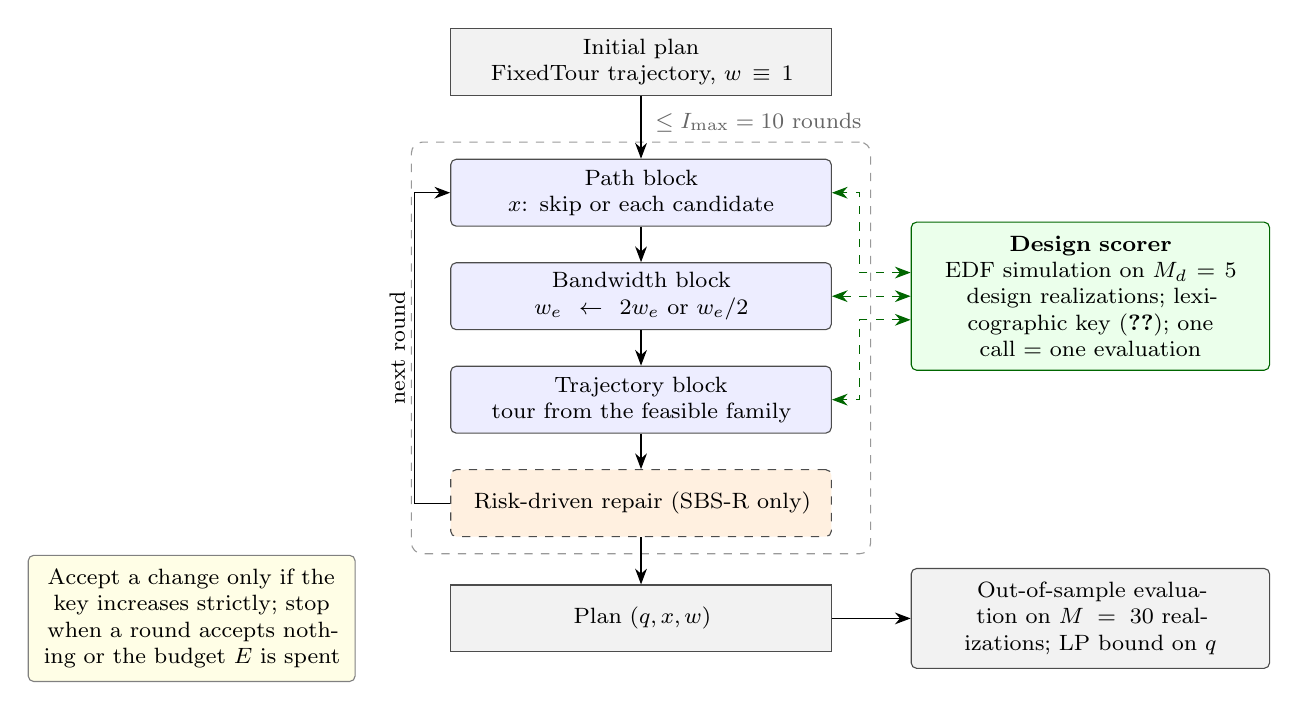
\begin{tikzpicture}[>={Stealth[length=2mm]}, node distance=0.45cm,
    blk/.style={draw=black!70, rounded corners=2pt, fill=blue!7, text width=4.6cm, minimum height=0.85cm, align=center, font=\footnotesize},
    rep/.style={blk, fill=orange!12, dashed},
    io/.style={draw=black!70, fill=black!5, text width=4.6cm, minimum height=0.85cm, align=center, font=\footnotesize},
    sc/.style={draw=green!40!black, rounded corners=2pt, fill=green!8, text width=4.2cm, align=center, font=\footnotesize, inner sep=5pt}]
  \node[io] (init) {Initial plan\\FixedTour trajectory, $w\equiv 1$};
  \node[blk, below=0.8cm of init] (path) {Path block\\$x$: skip or each candidate};
  \node[blk, below=of path] (bw) {Bandwidth block\\$w_e\gets 2w_e$ or $w_e/2$};
  \node[blk, below=of bw] (traj) {Trajectory block\\tour from the feasible family};
  \node[rep, below=of traj] (repair) {Risk-driven repair (SBS-R only)};
  \node[io, below=0.6cm of repair] (out) {Plan $(q,x,w)$};
  \node[sc, right=1.0cm of bw] (scorer) {\textbf{Design scorer}\\EDF simulation on $M_d=5$ design realizations; lexicographic key \eqref{eq:objective}; one call $=$ one evaluation};
  \node[sc, right=1.0cm of out, fill=black!5, draw=black!70] (eval) {Out-of-sample evaluation on $M=30$ realizations; LP bound on $q$};
  \node[sc, left=1.2cm of out, text width=3.8cm, fill=yellow!10, draw=black!50] (rule) {Accept a change only if the key increases strictly; stop when a round accepts nothing or the budget $E$ is spent};
  \draw[->] (init) -- (path);
  \draw[->] (path) -- (bw);
  \draw[->] (bw) -- (traj);
  \draw[->] (traj) -- (repair);
  \draw[->] (repair) -- (out);
  \draw[->] (out) -- (eval);
  \draw[->] (repair.west) -- ++(-0.45,0) |- node[pos=0.25, sloped, above, font=\footnotesize] {next round} (path.west);
  \draw[<->, dashed, green!40!black] (scorer.west) ++(0,0.3) -- ++(-0.65,0) |- (path.east);
  \draw[<->, dashed, green!40!black] (scorer.west) -- (bw.east);
  \draw[<->, dashed, green!40!black] (scorer.west) ++(0,-0.3) -- ++(-0.65,0) |- (traj.east);
  \begin{scope}[on background layer]
    \node[draw=black!40, dashed, rounded corners=4pt, fit=(path)(bw)(traj)(repair), inner xsep=14pt, inner ysep=6pt, label={[font=\footnotesize, text=black!60, anchor=south east]north east:$\le I_{\max}=10$ rounds}] (loop) {};
  \end{scope}
\end{tikzpicture}
\caption{Pipeline of the proposed block search.}
\label{fig:pipeline}
\end{figure}

\subsection{Design Rationale}
\label{sec:algorithm}

We keep the three-block structure of~\cite{huang2025ddatsap} but do not solve each block as a convex problem, a choice motivated by three preliminary tests on six evaluation scenarios with ten realizations each. When the bandwidths of the solution of Problem (P2) were used as a static schedule, the timely-delivery ratio fell from \num{0.410} for the fixed-trajectory baseline FixedTour to \num{0.128}; used as bandwidth-sharing weights, they reached \num{0.404}, and paths taken from the solution of (P2) reached \num{0.412}. Guidance from the LP therefore does not carry over to the EDF scheduler, and under the PrLoS channel the trajectory block admits no valid convex surrogate for an objective that counts alerts. Local search scored by the evaluator itself, by contrast, raised the ratio to \num{0.427} when scoring on expected rates and to \num{0.449} when scoring on five sampled realizations, while scoring on expected rates even lowered one scenario from \num{0.372} to \num{0.305}. We therefore implement each block as an evaluated local-search step. Compared with a surrogate-based decomposition, this design measures every accepted change on the exact objective and scheduler used for evaluation, and it requires only samples of the channel rather than a convex surrogate of it.

\subsection{Plan Representation and Design Scoring}
\label{sec:weights}

A plan carries a weight $w_{e,n}\ge 0$ for every radio link $e$ and slot $n$ instead of an explicit bandwidth schedule. In each phase of a slot, let $\mathcal B_n$ be the set of access links with queued data, or the set of at most two downlinks whose queue heads have the earliest deadlines. As illustrated in \cref{fig:slot}, the bandwidth allocated to a link $e\in\mathcal B_n$ is
\begin{equation}
\label{eq:weights}
b_{e,n}=B_{\mathrm{tot}}\frac{w_{e,n}}{\sum_{e'\in\mathcal B_n}w_{e',n}},
\end{equation}
\noindent with equal sharing when the weights sum to $0$. The equal-sharing rule of the baselines is the special case in which all weights equal $1$. The weights are fixed before the mission, whereas the actual bandwidth depends only on the current queues, so the policy uses no future information. Unlike a static bandwidth schedule, which falls out of step with how the EDF scheduler serves the queues, this rule follows the backlog in every slot while still letting the search shift spectrum toward specific links.

\begin{figure}[htbp]
\centering
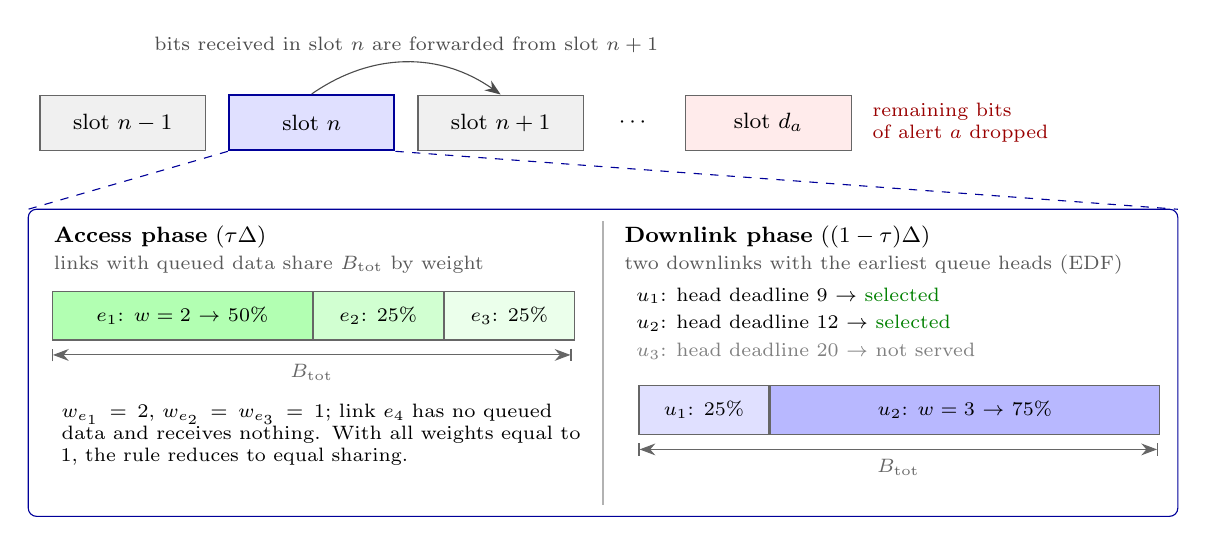
\begin{tikzpicture}[x=1cm, y=1cm, >={Stealth[length=2mm]},
    slot/.style={draw=black!60, fill=black!6, minimum width=2.1cm, minimum height=0.7cm, font=\footnotesize},
    seg/.style={draw=black!60, minimum height=0.62cm, font=\scriptsize, inner sep=1pt},
    lbl/.style={font=\footnotesize, align=center},
    small/.style={font=\scriptsize, align=left}]
  % slot timeline
  \node[slot] (s1) at (1.2,0) {slot $n-1$};
  \node[slot, fill=blue!12, draw=blue!60!black, thick] (s2) at (3.6,0) {slot $n$};
  \node[slot] (s3) at (6.0,0) {slot $n+1$};
  \node[lbl] at (7.7,0) {$\cdots$};
  \node[slot, fill=red!8] (s4) at (9.4,0) {slot $d_a$};
  \draw[->, black!70] (s2.north) to[bend left=35] node[above, small] {bits received in slot $n$ are forwarded from slot $n+1$} (s3.north);
  \node[small, text=red!60!black, anchor=west] at (10.6,0) {remaining bits\\of alert $a$ dropped};
  % zoom box
  \draw[blue!60!black, dashed] (s2.south west) -- (0,-1.1);
  \draw[blue!60!black, dashed] (s2.south east) -- (14.6,-1.1);
  \draw[draw=blue!60!black, rounded corners=3pt] (0,-1.1) rectangle (14.6,-5.0);
  % access phase
  \node[lbl, anchor=west] at (0.2,-1.45) {\textbf{Access phase} ($\tau\Delta$)};
  \node[small, anchor=west, text=black!65] at (0.2,-1.8) {links with queued data share $B_{\mathrm{tot}}$ by weight};
  \node[seg, fill=green!30, minimum width=3.3cm, anchor=west] (a1) at (0.3,-2.45) {$e_1$: $w=2$ $\to$ 50\%};
  \node[seg, fill=green!18, minimum width=1.65cm, anchor=west] (a2) at (a1.east) {$e_2$: 25\%};
  \node[seg, fill=green!8, minimum width=1.65cm, anchor=west] (a3) at (a2.east) {$e_3$: 25\%};
  \draw[|<->|, black!60] (0.3,-2.95) -- node[below, small] {$B_{\mathrm{tot}}$} (6.9,-2.95);
  \node[small, anchor=north west, text width=6.6cm] at (0.3,-3.45) {$w_{e_1}=2$, $w_{e_2}=w_{e_3}=1$; link $e_4$ has no queued data and receives nothing. With all weights equal to $1$, the rule reduces to equal sharing.};
  % downlink phase
  \draw[black!30] (7.3,-1.25) -- (7.3,-4.85);
  \node[lbl, anchor=west] at (7.45,-1.45) {\textbf{Downlink phase} ($(1-\tau)\Delta$)};
  \node[small, anchor=west, text=black!65] at (7.45,-1.8) {two downlinks with the earliest queue heads (EDF)};
  \node[small, anchor=west] (q1) at (7.6,-2.2) {$u_1$: head deadline $9$ $\to$ \textcolor{green!50!black}{selected}};
  \node[small, anchor=west] (q2) at (7.6,-2.55) {$u_2$: head deadline $12$ $\to$ \textcolor{green!50!black}{selected}};
  \node[small, anchor=west, text=black!50] (q3) at (7.6,-2.9) {$u_3$: head deadline $20$ $\to$ not served};
  \node[seg, fill=blue!12, minimum width=1.65cm, anchor=west] (d1) at (7.75,-3.65) {$u_1$: 25\%};
  \node[seg, fill=blue!28, minimum width=4.95cm, anchor=west] (d2) at (d1.east) {$u_2$: $w=3$ $\to$ 75\%};
  \draw[|<->|, black!60] (7.75,-4.15) -- node[below, small] {$B_{\mathrm{tot}}$} (14.35,-4.15);
\end{tikzpicture}
\caption{Slot structure and weighted bandwidth sharing with illustrative values.}
\label{fig:slot}
\end{figure}

\label{sec:scoring}
The search never uses the evaluation realizations. It scores a plan on $M_d=5$ design realizations, drawn from a random stream distinct from the evaluation stream, by summing the lexicographic key \eqref{eq:objective} over these realizations. Each scoring call counts as one evaluation, and the total number of evaluations is capped by a budget $E=2000$; when the budget is exhausted, the method returns the best plan found so far. A change is accepted only if the key increases strictly, so the key of the current plan never decreases. During design scoring, the independent ledger checker is skipped and $\mathrm{Conn}$ is cached per trajectory and realization, since neither affects the search decisions; this leaves the returned plan unchanged and speeds up the search by a factor of about \num{2.9}. The final evaluation on the evaluation realizations still runs the checker.

The true objective is the expectation of the lexicographic key over the channel distribution. Summing the key over $M_d$ design realizations is a sample average approximation (SAA) of this expectation with sample size $M_d=5$, whereas scoring on expected rates corresponds to the deterministic equivalent problem. Because design and evaluation realizations come from different random streams, all reported timely-delivery ratios are out-of-sample estimates. Our experiments on the number of design realizations examine the sample size of this SAA.

\subsection{Block Search and Schedule Repair}
\label{sec:b2}
SBS starts from the plan of FixedTour with all weights equal to $1$ and performs at most ten rounds of three blocks. The path block visits the alerts in increasing order of deadline and tries, in turn, leaving each alert unserved and assigning it to each of its candidates. The bandwidth block visits the radio links in use in decreasing order of the total size of the alerts they carry and tries to multiply all weights of a link by $2$, or by $1/2$ if doubling is rejected. The trajectory block scans the family of tours illustrated in \cref{fig:tours}, which are feasible by construction: the UAV leaves the center, flies in straight lines at speed $V_{\max}$ through an ordered subset of the damage zones, hovers at each stop, and returns. The remaining time is split among the stops equally, in proportion to the number of alerts of each zone, or in proportion to the sum of $1/(d_a-r_a)$ over the zone, and each stop is either the zone center or the centroid of the sources in the zone. With three zones, the family contains at most $90$ tours, including the trajectory of FixedTour. The search stops when a round accepts no change. Restricting the trajectory to this family gives up the continuous freedom of SCA-based trajectory design, but in return every candidate tour satisfies \eqref{eq:mobility} and can be evaluated directly on the exact objective.

\begin{figure}[htbp]
\centering
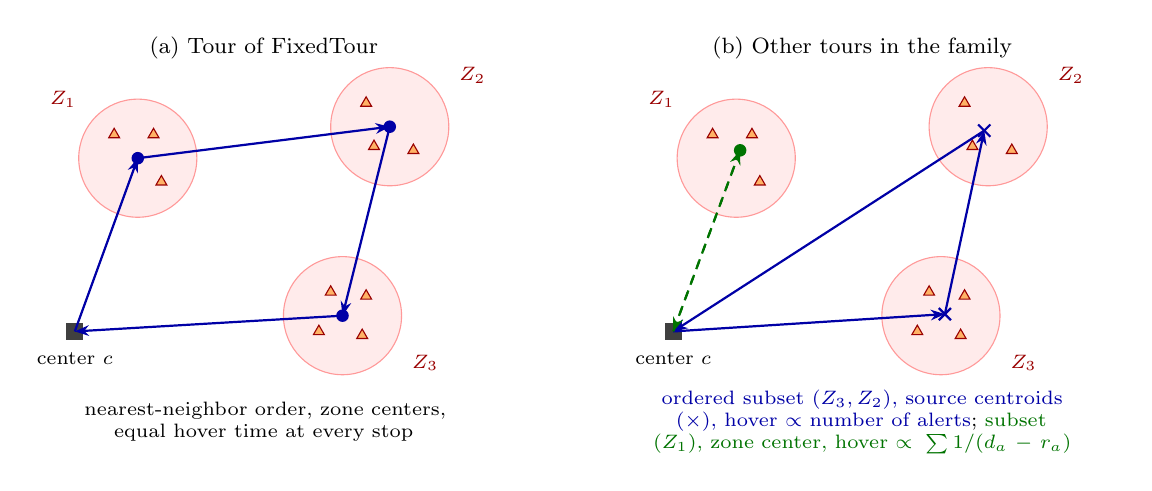
\begin{tikzpicture}[x=1cm, y=1cm, >={Stealth[length=1.8mm]},
    zone/.style={circle, fill=red!8, draw=red!40, minimum size=1.5cm},
    ctr/.style={rectangle, fill=black!75, minimum size=6pt, inner sep=0pt},
    src/.style={regular polygon, regular polygon sides=3, fill=orange!60, draw=red!60!black, inner sep=0.8pt},
    stopc/.style={circle, fill=blue!65!black, inner sep=1.6pt},
    stopg/.style={cross out, draw=blue!65!black, thick, inner sep=1.8pt},
    lbl/.style={font=\footnotesize, align=center},
    small/.style={font=\scriptsize, align=center}]
  \foreach \ox/\title in {0/{(a) Tour of FixedTour}, 7.6/{(b) Other tours in the family}} {
    \begin{scope}[shift={(\ox,0)}]
      \node[lbl] at (3.0,4.0) {\title};
      \node[zone] (Z1) at (1.4,2.6) {};
      \node[zone] (Z2) at (4.6,3.0) {};
      \node[zone] (Z3) at (4.0,0.6) {};
      \node[small, text=red!60!black] at (0.45,3.35) {$Z_1$};
      \node[small, text=red!60!black] at (5.65,3.65) {$Z_2$};
      \node[small, text=red!60!black] at (5.05,0.0) {$Z_3$};
      \foreach \p in {(1.1,2.9),(1.7,2.3),(1.6,2.9),(4.3,3.3),(4.9,2.7),(4.4,2.75),(3.7,0.4),(4.3,0.85),(4.25,0.35),(3.85,0.9)} \node[src] at \p {};
      \node[ctr] (c) at (0.6,0.4) {};
      \node[small, anchor=north] at (0.6,0.25) {center $c$};
    \end{scope}
  }
  % (a) nearest-neighbor tour through all zone centers, equal hover
  \draw[->, blue!65!black, thick] (0.6,0.4) -- (1.4,2.6);
  \draw[->, blue!65!black, thick] (1.4,2.6) -- (4.6,3.0);
  \draw[->, blue!65!black, thick] (4.6,3.0) -- (4.0,0.6);
  \draw[->, blue!65!black, thick] (4.0,0.6) -- (0.6,0.4);
  \foreach \p in {(1.4,2.6),(4.6,3.0),(4.0,0.6)} \node[stopc] at \p {};
  \node[small, text width=5.6cm] at (3.0,-0.75) {nearest-neighbor order, zone centers,\\equal hover time at every stop};
  % (b) two alternative tours
  \begin{scope}[shift={(7.6,0)}]
    \draw[->, blue!65!black, thick] (0.6,0.4) -- (4.05,0.62);
    \draw[->, blue!65!black, thick] (4.05,0.62) -- (4.55,2.95);
    \draw[->, blue!65!black, thick] (4.55,2.95) -- (0.6,0.4);
    \node[stopg] at (4.05,0.62) {};
    \node[stopg] at (4.55,2.95) {};
    \draw[->, green!45!black, thick, dashed] (0.6,0.4) -- (1.45,2.7);
    \draw[->, green!45!black, thick, dashed] (1.45,2.7) -- (0.6,0.4);
    \node[stopc, fill=green!45!black] at (1.45,2.7) {};
    \node[small, text width=6.4cm] at (3.0,-0.75) {\textcolor{blue!65!black}{ordered subset $(Z_3,Z_2)$, source centroids ($\times$), hover $\propto$ number of alerts}; \textcolor{green!45!black}{subset $(Z_1)$, zone center, hover $\propto\sum 1/(d_a-r_a)$}};
  \end{scope}
\end{tikzpicture}
\caption{Family of feasible tours scanned by the trajectory block.}
\label{fig:tours}
\end{figure}

\label{sec:repair}
The blocks of SBS change one decision at a time without regard to which alerts are about to miss their deadlines. SBS-R targets these alerts directly by adding a repair loop after the trajectory block of every round, as illustrated in \cref{fig:repair}. A ledger evaluation of the current plan records, for each alert and design realization, its slack $d_a-1-t_a$, where $t_a$ is the completion slot and the slack is set to $-1$ for late alerts, together with the hop that holds the alert's data for the most slots and the links whose capacity is exhausted. The risk of an alert is the fraction of design realizations in which it is late or has a slack of at most $\theta=2$ slots, and the loop considers at most $R=10$ alerts with the highest risk. If the bottleneck hop of such an alert is a radio link, Operator~1 doubles its weight within the slots $[r_a,d_a)$ only, which moves bandwidth from the other links of the same phase to this alert. Operator~2 tries the other candidates of the alert, ranked first by the number of congested links in its window and then by estimated cost, and accepts the first one that increases the key. All operators share the budget with the three blocks, so SBS-R and SBS have the same maximum number of evaluations. The mechanism follows the destroy-and-repair principle of large neighborhood search~\cite{ropke2006alns}.

\begin{figure}[htbp]
\centering
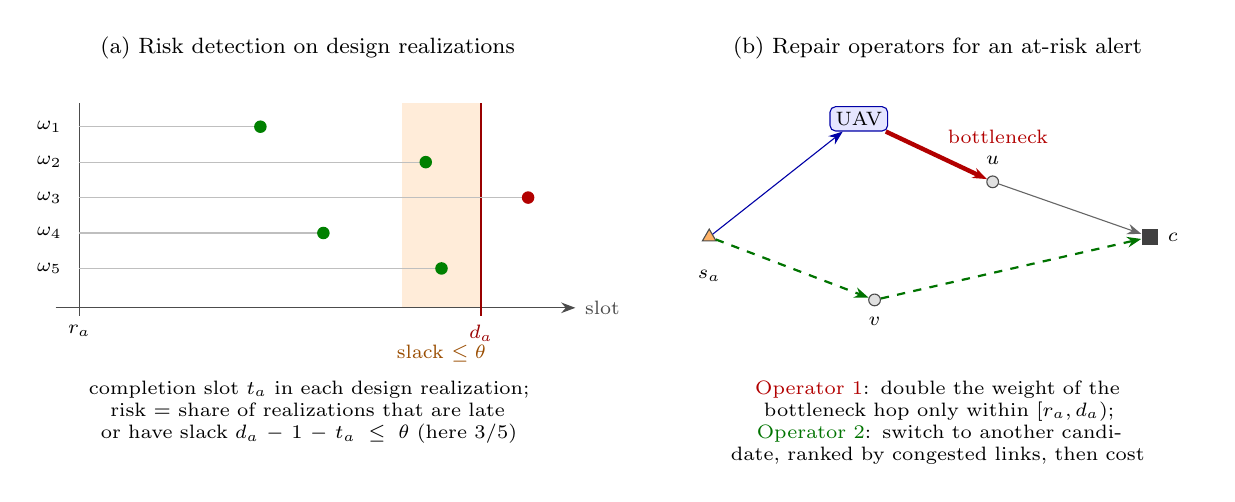
\begin{tikzpicture}[x=1cm, y=1cm, >={Stealth[length=1.8mm]},
    lbl/.style={font=\footnotesize, align=center},
    small/.style={font=\scriptsize, align=center},
    nd/.style={circle, draw=black!70, fill=black!12, inner sep=1.5pt},
    late/.style={circle, fill=red!70!black, inner sep=1.6pt},
    ontime/.style={circle, fill=green!50!black, inner sep=1.6pt}]
  % (a) risk detection
  \node[lbl] at (3.2,3.3) {(a) Risk detection on design realizations};
  \fill[orange!15] (4.4,0.0) rectangle (5.4,2.6);
  \draw[->, black!70] (0,0) -- (6.6,0) node[right, small] {slot};
  \draw[black!70] (0.3,-0.1) -- (0.3,2.6); \node[small, anchor=north] at (0.3,-0.1) {$r_a$};
  \draw[red!60!black, thick] (5.4,-0.1) -- (5.4,2.6); \node[small, anchor=north, text=red!60!black] at (5.4,-0.1) {$d_a$};
  \node[small, anchor=north, text=orange!60!black] at (4.9,-0.35) {slack $\le\theta$};
  \foreach \y/\x/\st [count=\i] in {2.3/2.6/ontime, 1.85/4.7/ontime, 1.4/6.0/late, 0.95/3.4/ontime, 0.5/4.9/ontime} {
    \node[small, anchor=east] at (0.2,\y) {$\omega_{\i}$};
    \draw[black!25] (0.3,\y) -- (\x,\y);
    \node[\st] at (\x,\y) {};
  }
  \node[small, text width=6.4cm, anchor=north] at (3.2,-0.8) {completion slot $t_a$ in each design realization; risk $=$ share of realizations that are late or have slack $d_a-1-t_a\le\theta$ (here $3/5$)};
  % (b) operators
  \begin{scope}[shift={(8.0,0)}]
    \node[lbl] at (3.2,3.3) {(b) Repair operators for an at-risk alert};
    \node[nd, fill=orange!60, regular polygon, regular polygon sides=3, inner sep=1pt] (s) at (0.3,0.9) {};
    \node[small, anchor=north] at (0.3,0.6) {$s_a$};
    \node[draw=blue!65!black, fill=blue!10, rounded corners=2pt, font=\scriptsize, inner sep=2pt] (uav) at (2.2,2.4) {UAV};
    \node[nd] (u) at (3.9,1.6) {}; \node[small, anchor=south] at (3.9,1.7) {$u$};
    \node[nd] (v) at (2.4,0.1) {}; \node[small, anchor=north] at (2.4,0.0) {$v$};
    \node[rectangle, fill=black!75, minimum size=6pt, inner sep=0pt] (c) at (5.9,0.9) {}; \node[small, anchor=west] at (6.0,0.9) {$c$};
    \draw[->, blue!65!black] (s) -- (uav);
    \draw[->, red!70!black, line width=1.6pt] (uav) -- node[above right, small, text=red!70!black] {bottleneck} (u);
    \draw[->, black!60] (u) -- (c);
    \draw[->, green!45!black, dashed, thick] (s) -- (v);
    \draw[->, green!45!black, dashed, thick] (v) -- (c);
    \node[small, text width=6.6cm, anchor=north] at (3.2,-0.8) {\textcolor{red!70!black}{Operator 1}: double the weight of the bottleneck hop only within $[r_a,d_a)$;\\ \textcolor{green!45!black}{Operator 2}: switch to another candidate, ranked by congested links, then cost};
  \end{scope}
\end{tikzpicture}
\caption{Risk-driven schedule repair in SBS-R: (a)~risk detection; (b)~repair operators.}
\label{fig:repair}
\end{figure}

\subsection{Overall Algorithm and Complexity}
\label{sec:overall}

\Cref{alg:bcd-repair} summarizes the method; SBS is obtained with repair disabled and SBS-R with repair enabled.

\begin{algorithm}[htbp]
\caption{Sample-scored block search with schedule repair.}
\label{alg:bcd-repair}
\begin{algorithmic}[1]
\Require Scenario, candidate set, design realizations, budget $E$, maximum rounds $I_{\max}=10$
\Ensure Trajectory $q$, path selection $x$, bandwidth weights $w$
\State $(q,x)\gets$ plan of FixedTour; $w\gets 1$; $\kappa\gets$ key of $(q,x,w)$
\For{$i=1,\dots,I_{\max}$}
    \State Path block: for each alert in deadline order, try skipping it and each candidate
    \State Bandwidth block: for each link in use, try $w_e\gets 2w_e$, then $w_e\gets w_e/2$
    \State Trajectory block: try each tour in the family of feasible tours
    \If{repair is enabled}
        \State Ledger evaluation; select at most $R$ alerts with the highest deadline risk
        \ForAll{at-risk alerts $a$}
            \State Operator 1: double the weight of the bottleneck hop within $[r_a,d_a)$
            \State Operator 2: try other candidates by number of congested links, then by cost
        \EndFor
    \EndIf
    \State Accept each trial iff the key increases strictly; stop as soon as the budget $E$ is spent
    \If{no change was accepted in this round} \textbf{break} \EndIf
\EndFor
\State \Return $(q,x,w)$
\end{algorithmic}
\end{algorithm}

One round uses at most $(K+1)\abs{A}+2\abs{\mathcal L_{\mathrm{used}}}+90$ evaluations for the three blocks plus $1+RK$ for the repair loop of SBS-R, where $\mathcal L_{\mathrm{used}}$ is the set of radio links in use. Each evaluation costs $O\bigl(M_dN(\abs{\mathcal L}+\abs{A}\log\abs{A})\bigr)$, and risk detection scans the ledger in $O\bigl(M_d(N\abs{\mathcal L}+T)\bigr)$, where $T$ is the number of transmission records. The budget caps the total number of evaluations, so the planning time of SBS, SBS-Lex, and SBS-R is $O\bigl(EM_dN(\abs{\mathcal L}+\abs{A}\log\abs{A})\bigr)$, independent of the actual number of rounds. The method only guarantees that the key of the plan does not decrease; it does not guarantee optimality, and the LP bound (P2), solved on the trajectory chosen by each method, measures the remaining room for improvement.

\label{sec:variants}
To separate the effect of the objective from that of the search, SBS-Lex runs the same search as SBS with a different key. Let $\bar f_a$ be the fraction of the bits of $a$ that reach the center before the deadline, averaged over the design realizations. The average delivery rate of $a$ divided by its required rate $L_a/((d_a-r_a)\Delta)$ equals exactly $\bar f_a$, so $\min_a \bar f_a$ is a normalized version of the max--min objective of~\cite{huang2025ddatsap}. Because a single undeliverable alert forces $\min_a\bar f_a=0$ for every plan, SBS-Lex compares plans in leximin order:
\begin{equation}
\label{eq:leximin}
\bigl(\bar f_{(1)},\bar f_{(2)},\dots,\bar f_{(\abs{A})},\ \textstyle\sum_{\omega}\sum_a z_{a,\omega},\ \mathrm{Conn}\bigr),\qquad \bar f_{(1)}\le\bar f_{(2)}\le\dots\le\bar f_{(\abs{A})},
\end{equation}
\noindent where an unserved alert has $\bar f_a=0$. The difference between SBS and SBS-Lex measures the cost of optimizing fairness instead of the number of timely alerts.

\section{Numerical Results}
\label{sec:experiments}

This section evaluates the proposed algorithm in simulation. The experiments address four questions: whether jointly optimizing trajectory, paths, and bandwidth improves the timely-delivery ratio over partial optimization and over a strong method from the literature, which design choices produce the gain, when the UAV matters, and whether the conclusions survive parameter changes and a realistic source layout.

\subsection{Simulation Setup}
\label{sec:setup}
The first scenario family, called Wide, is generated deterministically from the 130 Topology Zoo topologies that have between 15 and 40 nodes, geographic coordinates, and a connected graph. After stratifying them by node count, we use ten topologies for evaluation with three replicates each and reserve three others for development with two replicates each. Alert sizes inherit their relative proportions from the demands of the SNDlib instance \texttt{abilene}~\cite{orlowski2010sndlib}, whereas damage zones, source positions, release times, deadlines, and failed edges are drawn from seeded random streams. The second family, called Narrow, keeps every seed and only lowers the backhaul capacity from \qty{1000}{\kilo\bit\per\second} to \qty{50}{\kilo\bit\per\second}, so that both families share the same topologies, alerts, and failure patterns. \Cref{tab:params} lists the simulation parameters, whose channel constants follow those of~\cite{huang2025ddatsap}. All scenarios are synthesized from public data and do not represent measured rescue networks.

% Parameter table — rows read from data/params.csv (written by experiments/report_tables.py).
\begin{table}[htbp]
\centering
\small
\setlength{\tabcolsep}{4pt}
\caption{Simulation parameters.}
\label{tab:params}
\begin{tabular}{@{}lll@{}}
\toprule
\textbf{Parameter} & \textbf{Symbol} & \textbf{Value} \\
\midrule
\csvreader[separator=semicolon, late after line=\\]{data/params.csv}{1=\colparameter, 2=\colsymbol, 3=\colvalue}{\colparameter & \colsymbol & \colvalue}
\bottomrule
\end{tabular}
\end{table}


\label{sec:rescuenet}
For the case study, the sources are instead placed at damaged buildings in the RescueNet dataset~\cite{rahnemoonfar2023rescuenet}, which contains UAV images of Mexico Beach taken after Hurricane Michael together with segmentation masks. On \ResultExtImageCount{} image--mask pairs, we extract the 8-connected regions labeled as minor damage, major damage, or total destruction, discard those smaller than \qty{10}{\metre\squared}, and represent each remaining region by its pixel closest to the centroid. Because the dataset does not report the ground sampling distance, we derive the pixel size from the altitude and calibrated focal length stored in the image metadata, which gives values between \ResultExtGsdMin{} and \ResultExtGsdMax~\unit{\centi\metre}, and we project every point into UTM zone 16N using the GPS position and gimbal orientation. Merging points from overlapping images that lie within \qty{10}{\metre} of each other reduces the \ResultExtRegionCount{} damaged regions to \ResultExtTargetCount{} targets, which are then normalized into a \qty{2}{\kilo\metre} region with the same scale on both axes.

The resulting family, called RescueNet, follows every other rule of Wide: it uses the same ten evaluation topologies, three replicates, and random streams for alerts and failed edges, but every target becomes a source and the three damage zones are obtained by k-means clustering of the targets. Since the targets spread over the whole region rather than clustering around three centers, only \ResultExtGroundFractionRescuenet{} of the sources have a ground relay in range, compared with \ResultExtGroundFractionVzero{} in Wide. All targets come from a single geographic layout observed in overlapping images, so we report the case-study results descriptively.

\label{sec:baselines}
We compare the proposed methods SBS and SBS-R with the following benchmark schemes:
\begin{itemize}
\item NoUAV: only ground paths are used.
\item FixedTour: the UAV follows a fixed tour of the damage zones, and paths are chosen per alert.
\item SBS-Lex: the search of SBS with the fairness key \eqref{eq:leximin}.
\item Tran-IA: the inner approximation algorithm of Tran et al.~\cite{tran2022relay}, adapted to our model as described below.
\end{itemize}
NoUAV and FixedTour share the candidate set, the EDF scheduler, and equal bandwidth sharing, and both plan from expected rates. NoUAV routes each alert over its lowest-cost ground path and leaves an alert unserved when its source has no relay in range, at a planning cost of $O(\abs{A}K)$. FixedTour flies the UAV to the zone centers in nearest-neighbor order with equal hover times, as shown in \cref{fig:tours}a, and assigns each alert to the candidate that completes earliest when simulated alone on this trajectory; an alert is left unserved if no candidate meets its deadline. Its planning cost is $O(\abs{A}KNH_{\max})$, where $H_{\max}$ is the largest number of hops of a candidate.

\label{sec:tran}
Tran-IA, the half-duplex algorithm of Tran et al.~\cite{tran2022relay}, maximizes the number of devices whose data are uploaded to the UAV within an upload window and then offloaded to a gateway, with a binary variable $\lambda_k$ indicating whether device $k$ is served. The algorithm relaxes $\lambda_k$ to $[0,1]$ and adds the penalty $\mu\sum_k\lambda_k(\lambda_k-1)$; each iteration then linearizes the penalty, replaces the rates by concave lower bounds around the current point, and solves a convex problem in trajectory, bandwidth, and $\lambda$. \Cref{tab:tran-adaptation} lists the changes required by our model. They preserve the structure of the algorithm but may put it at a disadvantage, because the original work models neither a finite backhaul nor an EDF scheduler.

% Tran-IA adaptation — hand-written table (spec D Section 5.1).
\begin{table}[htbp]
\centering
\small
\caption{Adaptation of Tran-IA to our model.}
\label{tab:tran-adaptation}
\begin{tabularx}{\textwidth}{@{}>{\raggedright\arraybackslash}p{0.38\textwidth}>{\raggedright\arraybackslash}X@{}}
\toprule
\textbf{Original paper} & \textbf{This work} \\
\midrule
Device $k$ with $S_k$ bits, a start time, and an upload deadline & Alert $a$ with $L_a$ bits, release slot $r_a$, and upload window $[r_a,\,r_a+\lceil\theta W_a\rceil)$ \\
One gateway; offloading from the upload deadline until the end of the mission & Gateway is the entry node of the lowest-cost candidate; offloading within $[r_a+\lceil\theta W_a\rceil,\,d_a-b_a)$ \\
Device and UAV powers optimized & Fixed powers, as for every method \\
Rician channel with path loss $\omega_0 d^{-\alpha}$ & Power law $\beta d^{-\alpha}$ fitted to the expected PrLoS gain \\
Finite UAV memory & None, since the UAV buffer is unlimited in our model \\
No limit on concurrent downlinks & At most two downlinks with the largest bandwidths kept per slot \\
Feasibility problem for initialization & Initialized from the FixedTour trajectory, equal bandwidths, and $\lambda=0$, which is always feasible \\
No values given for $\mu$ and the convergence threshold & $\theta$ and $\mu$ selected on the development set; stop when the objective changes by less than $10^{-3}$ or after 30 iterations \\
\bottomrule
\end{tabularx}
\end{table}


In the adapted version, each alert plays the role of a device, and its gateway is the node where its lowest-cost candidate enters the ground network. Given $b_a$ slots of backhaul delay and $W_a=d_a-b_a-r_a$, the upload window is $[r_a,\,r_a+\lceil\theta W_a\rceil)$ and the offloading window ends at $d_a-b_a$, which leaves enough time for the data to cross the backhaul before the deadline. The Rician channel of the original work is replaced by a power law $\beta d^{-\alpha}$ fitted by least squares to the expected PrLoS gain; on the development scenarios, the fitted exponent lies between \ResultExtFitAlphaMin{} and \ResultExtFitAlphaMax{} with $R^2$ of at least \ResultExtFitRsquaredMin. Each iteration solves a second-order cone program with \texttt{cvxpy} and Clarabel. The algorithm starts from the FixedTour trajectory with equal bandwidths and $\lambda=0$, stops when the relaxed objective changes by less than $10^{-3}$ or after 30 iterations, and converts its solution into a static bandwidth schedule that keeps at most two downlinks per slot. We selected $\theta=\ResultExtPilotTheta$ and $\mu=\ResultExtPilotMu$ on \ResultExtPilotScenarioCount{} development scenarios from the grid $\theta\in\{1/3,1/2,2/3\}$, $\mu\in\{1,10\}$, although all grid cells were within \ResultExtPilotGridSpread{} of each other in timely-delivery ratio.

\label{sec:protocol}
Each method plans once per scenario, and its plan is evaluated on 30 channel realizations with common random numbers. The development topologies were used only in a single preliminary run that confirmed $E=2000$ and $M_d=5$, and no parameter was tuned on the evaluation set. The main experiment runs NoUAV, FixedTour, SBS, SBS-Lex, SBS-R, Tran-IA, and seven ablation variants of SBS-R on the \ResultTwoScenarioCount{} evaluation scenarios of each family, and it solves the LP bound for every realization on the trajectory of each method. For each realization, the envelope bound is the largest of the bounds on the trajectories of FixedTour, SBS, SBS-Lex, and SBS-R, and the envelope gap of a method is measured against it in the same way as the gap to its own bound. The result tables report planning times in seconds and the mean number of evaluations used by the search. Two further experiments vary the budget $E$ from 250 to 4000 on Wide and vary one parameter at a time on the first replicate of each evaluation topology.

Results are averaged first over realizations and then over scenarios. Because the replicates of a topology are not independent, 95\% confidence intervals (CIs) are computed with a bootstrap clustered by topology, and paired comparisons are based on the ten topology-level differences. Each comparison uses an exact sign-flip test over all $2^{10}$ sign assignments, a bootstrap CI with \num{10000} resamples, and the matched-pairs rank-biserial correlation as effect size, and its $p$-value is Holm-corrected within its group, namely the eight comparisons among our methods or the four comparisons against Tran-IA. Ablation, sensitivity, and case-study results are reported descriptively. All bound LPs were solved to optimality with HiGHS. The implementation uses Python \ResultPythonVersion, \texttt{scipy} \ResultScipyVersion, HiGHS \ResultHighsVersion, \texttt{cvxpy}~\ResultExtCvxpyVersion, and Clarabel~\ResultExtClarabelVersion, runs \ResultWorkers{} worker processes on a \ResultCpuCount-CPU machine, and consumed \ResultExtComputeHours{} compute hours for all experiments together.

\subsection{Comparison with Benchmark Schemes}
\label{sec:results-main}

% Main comparison — rows read from data/phase2_main.csv (written by experiments/report_tables_phase2.py).
\begin{table}[htbp]
\centering
\footnotesize
\setlength{\tabcolsep}{3pt}
\caption{Main comparison on both scenario families.}
\label{tab:phase2-main}
\begin{tabular}{@{}llcccccrr@{}}
\toprule
\textbf{Backhaul} & \textbf{Method} & \textbf{Timely $\uparrow$} & \textbf{95\% CI} & \textbf{Conn $\uparrow$} & \textbf{Own gap $\downarrow$} & \textbf{Env.\ gap $\downarrow$} & \textbf{Plan.\ (s)} & \textbf{Eval.} \\
\midrule
\csvreader[separator=semicolon, late after line=\\]{data/phase2_main.csv}{2=\colbackhaul, 3=\colmethod, 4=\coltimely, 5=\colci, 6=\colconn, 7=\colgap, 8=\coluniongap, 9=\colplanning, 10=\colcalls}{\colbackhaul & \colmethod & \coltimely & \colci & \colconn & \colgap & \coluniongap & \colplanning & \colcalls}
\bottomrule
\end{tabular}
\end{table}


As \cref{tab:phase2-main} shows, jointly optimizing the plan pays off clearly over both baselines. On Wide, SBS delivers \ResultTwoTimelyVzeroBtwo{} of the alerts on time, against \ResultTwoTimelyVzeroBone{} for FixedTour and \ResultTwoTimelyVzeroBzero{} for NoUAV, and it outperforms NoUAV on \ResultTwoHigherVzeroBtwoBzero{} and FixedTour on \ResultTwoHigherVzeroBtwoBone{} of the \ResultTwoScenarioCount{} scenarios. The repair variant SBS-R reaches \ResultTwoTimelyVzeroP, practically the same as SBS: it is better on \ResultTwoHigherVzeroPBtwo{} scenarios, equal on \ResultTwoEqualVzeroPBtwo{}, and worse on \ResultTwoLowerVzeroPBtwo. SBS-Lex reaches only \ResultTwoTimelyVzeroBthree, below even FixedTour, although every method that uses the UAV brings connectivity close to one. Reducing the backhaul to \qty{50}{\kilo\bit\per\second} lowers all ratios but leaves the ranking unchanged, with SBS at \ResultTwoTimelyVzeroBhfivezeroBtwo, SBS-R at \ResultTwoTimelyVzeroBhfivezeroP, FixedTour at \ResultTwoTimelyVzeroBhfivezeroBone, and NoUAV at \ResultTwoTimelyVzeroBhfivezeroBzero.

The relative gaps to the upper bounds point in the same direction. The gap of SBS to the bound on its own trajectory is \ResultTwoGapVzeroBtwo, whereas that of FixedTour to the bound on the FixedTour trajectory is \ResultTwoGapVzeroBone, because SBS delivers more alerts and also chooses trajectories with higher bounds. Relative to the envelope bound of \ResultTwoUnionBoundVzeroBtwo, the gaps are \ResultTwoUnionGapVzeroBtwo{} for SBS and \ResultTwoUnionGapVzeroBone{} for FixedTour. SBS-Lex shows a gap of \ResultTwoGapVzeroBthree{} even though its trajectory has nearly the same bound as that of SBS, which indicates that its loss stems from the path and bandwidth choices made under the leximin objective rather than from the trajectory.

\label{sec:results-stats}
% Paired tests — rows read from data/phase2_statistics.csv (written by experiments/report_tables_phase2.py).
\begin{table}[htbp]
\centering
\small
\setlength{\tabcolsep}{4pt}
\caption{Paired comparisons with the baselines.}
\label{tab:phase2-stats}
\begin{tabular}{@{}llccccc@{}}
\toprule
\textbf{Family} & \textbf{Comparison} & \textbf{Difference} & \textbf{95\% CI} & \textbf{$r$} & \textbf{$p$} & \textbf{$p_{\mathrm{Holm}}$} \\
\midrule
\csvreader[separator=semicolon, late after line=\\]{data/phase2_statistics.csv}{1=\colset, 2=\colcomparison, 3=\coldiff, 4=\colci, 5=\colr, 6=\colp, 7=\colholm}{\colset & \colcomparison & \coldiff & \colci & \colr & \colp & \colholm}
\bottomrule
\end{tabular}
\end{table}


The paired tests in \cref{tab:phase2-stats} confirm that these differences are systematic. SBS exceeds FixedTour by \ResultTwoDiffVzeroBtwoBone{} on average on Wide, with a 95\% CI of [\ResultTwoDiffLowVzeroBtwoBone, \ResultTwoDiffHighVzeroBtwoBone], and by \ResultTwoDiffVzeroBhfivezeroBtwoBone{} on Narrow, while SBS-R exceeds FixedTour by \ResultTwoDiffVzeroPBone{} and \ResultTwoDiffVzeroBhfivezeroPBone, respectively. These comparisons and SBS $-$ SBS-Lex all reach $p_{\mathrm{Holm}}=\ResultTwoHolmFloor$, the smallest value attainable with ten topologies and eight comparisons, because all ten topologies agree in sign and the rank-biserial correlation equals one. The difference between SBS-R and SBS, in contrast, is only \ResultTwoDiffVzeroPBtwo{} on Wide, with a CI of [\ResultTwoDiffLowVzeroPBtwo, \ResultTwoDiffHighVzeroPBtwo] that contains zero, and \ResultTwoDiffVzeroBhfivezeroPBtwo{} on Narrow, with $p_{\mathrm{Holm}}=\ResultTwoHolmVzeroPBtwo$ in both cases; the data therefore provide no evidence that schedule repair improves on SBS.

\label{sec:results-literature}
% Comparison with TRAN — rows read from data/ext_literature.csv (written by experiments/report_tables_extensions.py).
\begin{table}[htbp]
\centering
\small
\setlength{\tabcolsep}{4pt}
\caption{Results of TRAN.}
\label{tab:literature}
\begin{tabular}{@{}llcccr@{}}
\toprule
\textbf{Backhaul} & \textbf{Method} & \textbf{Timely $\uparrow$} & \textbf{95\% CI} & \textbf{Gap $\downarrow$} & \textbf{Planning (s) $\downarrow$} \\
\midrule
\csvreader[separator=semicolon, late after line=\\, filter strcmp={\colmethod}{TRAN}]{data/ext_literature.csv}{2=\colbackhaul, 3=\colmethod, 4=\coltimely, 5=\colci, 6=\colgap, 7=\colplanning}{\colbackhaul & \colmethod & \coltimely & \colci & \colgap & \colplanning}
\bottomrule
\end{tabular}
\end{table}


\Cref{tab:literature} reports the results of Tran-IA, which can be read against those of FixedTour, SBS, and SBS-R in \cref{tab:phase2-main}. On Wide, Tran-IA delivers \ResultExtTimelyVzeroTRAN{} of the alerts on time, more than FixedTour at \ResultExtTimelyVzeroBone{} but fewer than SBS at \ResultExtTimelyVzeroBtwo{} and SBS-R at \ResultExtTimelyVzeroP. Under narrow backhaul, its ratio of \ResultExtTimelyVzeroBhfivezeroTRAN{} falls close to that of FixedTour at \ResultExtTimelyVzeroBhfivezeroBone{} and clearly below that of SBS at \ResultExtTimelyVzeroBhfivezeroBtwo. Tran-IA also lies farther from the bound on its own trajectory, with gaps of \ResultExtGapVzeroTRAN{} and \ResultExtGapVzeroBhfivezeroTRAN, and it plans longer than SBS-R, taking \ResultExtPlanningVzeroTRAN{} instead of \ResultExtPlanningVzeroP{} seconds per scenario on Wide.

% Tests against Tran-IA — rows read from data/ext_literature_statistics.csv (written by experiments/report_tables_extensions.py).
\begin{table}[htbp]
\centering
\small
\setlength{\tabcolsep}{4pt}
\caption{Paired comparisons with Tran-IA.}
\label{tab:literature-stats}
\begin{tabular}{@{}llccccc@{}}
\toprule
\textbf{Family} & \textbf{Comparison} & \textbf{Difference} & \textbf{95\% CI} & \textbf{$r$} & \textbf{$p$} & \textbf{$p_{\mathrm{Holm}}$} \\
\midrule
\csvreader[separator=semicolon, late after line=\\]{data/ext_literature_statistics.csv}{1=\colset, 2=\colcomparison, 3=\coldiff, 4=\colci, 5=\colr, 6=\colp, 7=\colholm}{\colset & \colcomparison & \coldiff & \colci & \colr & \colp & \colholm}
\bottomrule
\end{tabular}
\end{table}


\Cref{tab:literature-stats} quantifies these differences. On Wide, SBS-R exceeds Tran-IA by \ResultExtDiffVzeroPTran{} on average, with a CI of [\ResultExtDiffLowVzeroPTran, \ResultExtDiffHighVzeroPTran] and $p_{\mathrm{Holm}}=\ResultExtHolmVzeroPTran$; on Narrow, the advantage grows to \ResultExtDiffVzeroBhfivezeroPTran, with a CI of [\ResultExtDiffLowVzeroBhfivezeroPTran, \ResultExtDiffHighVzeroBhfivezeroPTran] and $p_{\mathrm{Holm}}=\ResultExtHolmVzeroBhfivezeroPTran$, and SBS behaves similarly. Under narrow backhaul, the bootstrap CI excludes zero and the rank-biserial correlation reaches \ResultExtRankBiserialVzeroBhfivezeroPTran, yet no difference remains significant at the 5\% level after Holm correction for the four comparisons. This pattern is consistent with the design of Tran-IA, which plans on a deterministic effective channel with a static bandwidth schedule and without knowledge of the backhaul capacity, and therefore loses most of its advantage when the backhaul is narrow.

\begin{figure}[htbp]
\centering
\begin{tikzpicture}
\begin{semilogxaxis}[
    width=0.75\textwidth, height=4.6cm, xmin=0.05, xmax=1000,
    xlabel={Mean planning time (s)}, ylabel={Timely-delivery ratio},
    grid=major, legend style={font=\footnotesize, at={(0.5,-0.42)}, anchor=north, legend columns=3, column sep=6pt},
    yticklabel style={/pgf/number format/fixed, /pgf/number format/precision=2},
]
\addplot[mark=*, color=blue!70!black] table[col sep=comma, x=planning, y=timely] {data/phase2_budget_b2.csv};
\addlegendentry{SBS, $E=250$--$4000$}
\addplot[mark=square*, dashed, color=red!70!black] table[col sep=comma, x=planning, y=timely] {data/phase2_budget_p.csv};
\addlegendentry{SBS-R, $E=250$--$4000$}
\addplot[only marks, mark=triangle*, mark size=3pt, color=green!50!black, nodes near coords, point meta=explicit symbolic,
    every node near coord/.append style={font=\footnotesize, anchor=south west}]
    table[col sep=comma, x=planning, y=timely, meta=method] {data/ext_quality_points.csv};
\addlegendentry{FixedTour and Tran-IA}
\end{semilogxaxis}
\end{tikzpicture}
\caption{Timely-delivery ratio versus planning time on Wide.}
\label{fig:quality-runtime}
\end{figure}

\Cref{fig:quality-runtime} places Tran-IA and FixedTour on the quality--runtime curves that SBS and SBS-R trace for budgets from 250 to 4000. Already with a budget of $E=500$, SBS reaches \ResultTwoBudgetBtwoFivezerozero, above Tran-IA, at a fraction of its planning time, and larger budgets move both SBS and SBS-R toward the saturation level examined below.

\subsection{Ablation and Algorithm Analysis}
\label{sec:results-ablation}

% Ablation of SBS-R — rows read from data/phase2_ablation.csv (written by experiments/report_tables_phase2.py).
\begin{table}[htbp]
\centering
\footnotesize
\setlength{\tabcolsep}{2pt}
\caption{Ablation of SBS-R.}
\label{tab:phase2-ablation}
\begin{tabular}{@{}lcccc@{}}
\toprule
& \multicolumn{2}{c}{\textbf{Wide}} & \multicolumn{2}{c}{\textbf{Narrow}} \\
\cmidrule(lr){2-3}\cmidrule(lr){4-5}
\textbf{Variant} & \textbf{Timely $\uparrow$} & \textbf{$\Delta$ vs.\ SBS-R [CI]} & \textbf{Timely $\uparrow$} & \textbf{$\Delta$ vs.\ SBS-R [CI]} \\
\midrule
\csvreader[separator=semicolon, late after line=\\]{data/phase2_ablation.csv}{1=\colvariant, 2=\coltimely, 3=\coldiff, 4=\coltimelybh, 5=\coldiffbh}{\colvariant & \coltimely & \coldiff & \coltimelybh & \coldiffbh}
\bottomrule
\end{tabular}
\end{table}


The ablation in \cref{tab:phase2-ablation} identifies where the gain comes from, with $\Delta$ denoting the topology-level mean difference in timely-delivery ratio between a variant and SBS-R. Disabling the path block changes the timely-delivery ratio of SBS-R by \ResultTwoAblationDiffVzeroPFixedPaths{} on Wide and \ResultTwoAblationDiffVzeroBhfivezeroPFixedPaths{} on Narrow, and disabling the trajectory block changes it by \ResultTwoAblationDiffVzeroPFixedTrajectory{} and \ResultTwoAblationDiffVzeroBhfivezeroPFixedTrajectory. Designing on expected rates instead of five sampled realizations changes it by \ResultTwoAblationDiffVzeroPExpectedDesign{} and \ResultTwoAblationDiffVzeroBhfivezeroPExpectedDesign, even though it plans much faster. The remaining variants, which keep only one repair operator, repair without backlog information, or skip the bandwidth block, stay within a few thousandths of SBS-R. The gain of the search therefore comes from selecting paths and trajectory jointly on sampled realizations, while the bandwidth weights and the repair operators matter little once the EDF scheduler shares bandwidth according to the backlog.

\label{sec:results-connectivity}
% By ground connectivity — rows read from data/phase2_connectivity.csv (written by experiments/report_tables_phase2.py).
\begin{table}[htbp]
\centering
\small
\setlength{\tabcolsep}{4pt}
\caption{Results by ground connectivity.}
\label{tab:phase2-connectivity}
\begin{tabular}{@{}llcccccc@{}}
\toprule
\textbf{Family} & \textbf{Ground-reachable} & \textbf{Scenarios} & \textbf{Conn B0} & \textbf{B0} & \textbf{B1} & \textbf{B2} & \textbf{B2 $-$ B0} \\
\midrule
\csvreader[separator=semicolon, late after line=\\]{data/phase2_connectivity.csv}{1=\colset, 2=\colgroup, 3=\colscenarios, 4=\colconn, 5=\colbzero, 6=\colbone, 7=\colbtwo, 8=\colgain}{\colset & \colgroup & \colscenarios & \colconn & \colbzero & \colbone & \colbtwo & \colgain}
\bottomrule
\end{tabular}
\end{table}


To see when the UAV matters, \cref{tab:phase2-connectivity} groups the scenarios by the fraction of sources that have a ground relay in range. Without a UAV, both the connectivity, listed as Conn NoUAV, and the timely-delivery ratio closely follow this fraction, the latter with correlation coefficients of \ResultTwoGroundCorrelationVzero{} on Wide and \ResultTwoGroundCorrelationVzeroBhfivezero{} on Narrow, since alerts from sources without a relay in range cannot be delivered at all. The UAV raises connectivity close to one in every group, and the gain of SBS over NoUAV remains nearly constant across groups, from \ResultTwoTercileGainVzeroLow{} to \ResultTwoTercileGainVzeroHigh{} on Wide. The UAV therefore helps even where most sources already reach a ground relay.

\label{sec:results-budget}
\begin{figure}[htbp]
\centering
\begin{tikzpicture}
\begin{semilogxaxis}[
    width=0.75\textwidth, height=4.6cm, log basis x=2,
    xlabel={Evaluation budget $E$}, ylabel={Timely-delivery ratio},
    xtick={250,500,1000,2000,4000}, xticklabels={250,500,1000,2000,4000},
    grid=major, legend pos=south east,
    yticklabel style={/pgf/number format/fixed, /pgf/number format/precision=3},
]
\addplot[mark=*, color=blue!70!black] table[col sep=comma, x=budget, y=timely] {data/phase2_budget_b2.csv};
\addlegendentry{SBS}
\addplot[mark=square*, dashed, color=red!70!black] table[col sep=comma, x=budget, y=timely] {data/phase2_budget_p.csv};
\addlegendentry{SBS-R}
\end{semilogxaxis}
\end{tikzpicture}
\caption{Timely-delivery ratio versus the evaluation budget on Wide.}
\label{fig:budget}
\end{figure}

\Cref{fig:budget} shows that the search saturates quickly. SBS reaches \ResultTwoBudgetBtwoTwofivezero{} with $E=250$ and \ResultTwoBudgetBtwoOnezerozerozero{} with $E=1000$, and it stays almost constant up to $E=4000$, where it reaches \ResultTwoBudgetBtwoFourzerozerozero, because the search stops after about \ResultTwoBudgetCallsBtwoFourzerozerozero{} evaluations on average, once a round accepts no further change. SBS-R follows the same trend, with \ResultTwoBudgetPTwofivezero, \ResultTwoBudgetPOnezerozerozero, and \ResultTwoBudgetPFourzerozerozero{} for the same budgets. The default budget $E=2000$ therefore lies in the saturated regime, and the lack of improvement of SBS-R over SBS cannot be attributed to an insufficient budget. The number of design realizations matters more than the budget. Running SBS-R on the first replicate of each Wide topology, designing on expected rates yields \ResultTwoDesignExpected, one realization \ResultTwoDesignOne, five realizations \ResultTwoDesignFive, and ten realizations \ResultTwoDesignOnezero, while the planning time grows from \ResultTwoDesignPlanningExpected{} to \ResultTwoDesignPlanningOnezero{} seconds.

\label{sec:results-milp}
% MILP cross-check — rows read from data/phase1_milp.csv (written by experiments/report_tables.py).
\begin{table}[htbp]
\centering
\footnotesize
\setlength{\tabcolsep}{3pt}
\caption{Tightness of the LP bound on reduced instances.}
\label{tab:phase1-milp}
\begin{tabular}{@{}lccccccc@{}}
\toprule
\textbf{Scenario} & \textbf{$|A|$} & \textbf{FixedTour} & \textbf{MILP plan} & \textbf{MILP} & \textbf{MILP bound} & \textbf{LP bound} & \textbf{Time (s)} \\
\midrule
\csvreader[separator=semicolon, late after line=\\]{data/phase1_milp.csv}{1=\colscenario, 2=\colalerts, 3=\colmethod, 4=\colplan, 5=\colincumbent, 6=\coldual, 7=\collp, 9=\colruntime}{\colscenario & \colalerts & \colmethod & \colplan & \colincumbent & \coldual & \collp & \colruntime}
\bottomrule
\end{tabular}
\end{table}


\Cref{tab:phase1-milp} compares the LP bound (P2) with the exact MILP (P3) on \ResultMilpCount{} reduced instances with ten alerts each, using the FixedTour trajectory and the first channel realization; HiGHS solved \ResultMilpOptimalCount{} of these MILPs to optimality. The plan built from the MILP solution is executed with the better of its own bandwidths and backlog-based equal sharing. On these instances, FixedTour attains the MILP optimum in \ResultMilpMethodAtOptimumCount{} cases and the plan built from the MILP solution in \ResultMilpPlanAtOptimumCount{} cases, so the gap between the LP bound and the achieved value comes mainly from relaxing the integrality of path selection. The bandwidth rule matters as well: taking the bandwidths directly from the MILP solution delivers only \ResultMilpStaticTotal{} timely alerts in total over the five instances, whereas keeping the solution paths and sharing bandwidth equally by backlog delivers \ResultMilpEqualSplitTotal, because a static bandwidth schedule falls out of step with how the EDF scheduler serves the queues. Finally, the envelope of ten tangents overestimates the rate by at most \ResultTangentOverestimateMax{} in relative terms on $[B_{\mathrm{tot}}/512, B_{\mathrm{tot}}]$. The gaps in \cref{tab:phase2-main} should therefore be read as upper bounds on the room for improvement, and the improvement that is actually achievable may be considerably smaller.

\label{sec:results-runtime}
In terms of computational cost, NoUAV plans almost instantly, and FixedTour needs \ResultPlanningVzeroBone{} seconds per Wide scenario on average because it simulates every candidate. SBS and SBS-R take \ResultTwoPlanningVzeroBtwo{} and \ResultTwoPlanningVzeroP{} seconds with \ResultTwoCallsVzeroBtwo{} and \ResultTwoCallsVzeroP{} evaluations on average, running \ResultWorkers{} processes in parallel, and evaluating one plan on one realization takes about \ResultEvaluationVzeroBone{} seconds. The \ResultLpCount{} LPs that bound NoUAV and FixedTour have a median of \ResultLpVariablesMedian{} and at most \ResultLpVariablesMax{} variables, and their solve time has a median of \ResultLpRuntimeMedian{} seconds and a maximum of \ResultLpRuntimeMax{} seconds.

\subsection{Sensitivity and RescueNet Case Study}
\label{sec:results-sensitivity}
\begin{figure}[htbp]
\centering
\begin{tikzpicture}
\begin{groupplot}[
    group style={group size=3 by 2, horizontal sep=1.2cm, vertical sep=1.7cm},
    width=0.34\textwidth, height=4.3cm, ymin=0.2, ymax=0.65, grid=major,
    tick label style={font=\scriptsize}, label style={font=\footnotesize},
    yticklabel style={/pgf/number format/fixed, /pgf/number format/precision=1},
    cycle list={{blue!70!black, mark=*}, {green!50!black, mark=triangle*}, {red!70!black, dashed, mark=square*}},
]
\nextgroupplot[xlabel={$L_{\mathrm{ref}}$ (kbit)}, ylabel={Timely-delivery ratio}, xmode=log, log basis x=2, xtick={125,250,500,1000}, xticklabels={125,250,500,1000}, legend to name=senslegend, legend columns=3]
\addplot table[col sep=comma, x=x, y=B1] {data/phase2_sensitivity_lref.csv}; \addlegendentry{FixedTour}
\addplot table[col sep=comma, x=x, y=B2] {data/phase2_sensitivity_lref.csv}; \addlegendentry{SBS}
\addplot table[col sep=comma, x=x, y=P] {data/phase2_sensitivity_lref.csv}; \addlegendentry{SBS-R}
\nextgroupplot[xlabel={$C_e$ (kbit/s)}, xmode=log, xtick={50,100,1000}, xticklabels={50,100,1000}]
\addplot table[col sep=comma, x=x, y=B1] {data/phase2_sensitivity_backhaul.csv};
\addplot table[col sep=comma, x=x, y=B2] {data/phase2_sensitivity_backhaul.csv};
\addplot table[col sep=comma, x=x, y=P] {data/phase2_sensitivity_backhaul.csv};
\nextgroupplot[xlabel={Mean deadline window (slots)}, xtick={20,40,80}]
\addplot table[col sep=comma, x=x, y=B1] {data/phase2_sensitivity_deadline.csv};
\addplot table[col sep=comma, x=x, y=B2] {data/phase2_sensitivity_deadline.csv};
\addplot table[col sep=comma, x=x, y=P] {data/phase2_sensitivity_deadline.csv};
\nextgroupplot[xlabel={$B_{\mathrm{tot}}$ (MHz)}, ylabel={Timely-delivery ratio}, xtick={0.5,1,2}]
\addplot table[col sep=comma, x=x, y=B1] {data/phase2_sensitivity_btot.csv};
\addplot table[col sep=comma, x=x, y=B2] {data/phase2_sensitivity_btot.csv};
\addplot table[col sep=comma, x=x, y=P] {data/phase2_sensitivity_btot.csv};
\nextgroupplot[xlabel={Number of alerts $\abs{A}$}, xtick={20,40,60}]
\addplot table[col sep=comma, x=x, y=B1] {data/phase2_sensitivity_alerts.csv};
\addplot table[col sep=comma, x=x, y=B2] {data/phase2_sensitivity_alerts.csv};
\addplot table[col sep=comma, x=x, y=P] {data/phase2_sensitivity_alerts.csv};
\nextgroupplot[xlabel={Number of candidates $K$}, xtick={2,3,5}]
\addplot table[col sep=comma, x=x, y=B1] {data/phase2_sensitivity_paths.csv};
\addplot table[col sep=comma, x=x, y=B2] {data/phase2_sensitivity_paths.csv};
\addplot table[col sep=comma, x=x, y=P] {data/phase2_sensitivity_paths.csv};
\end{groupplot}
\end{tikzpicture}

\pgfplotslegendfromname{senslegend}
\caption{Sensitivity of the timely-delivery ratio to the main parameters.}
\label{fig:sensitivity}
\end{figure}

\Cref{fig:sensitivity} varies one parameter at a time around the Wide setting on the first replicate of each evaluation topology; the middle point of each panel corresponds to Wide, except in the backhaul panel, where the right and left points are Wide and Narrow. FixedTour remains below SBS and SBS-R in every non-degenerate family. The advantage narrows with short deadlines, where FixedTour reaches \ResultTwoSensSensDeadlineShortBone{} and SBS-R \ResultTwoSensSensDeadlineShortP, and widens with long deadlines, where FixedTour reaches \ResultTwoSensSensDeadlineLongBone{} and SBS-R \ResultTwoSensSensDeadlineLongP. Larger alerts reduce the ratio of every method sharply; with $L_{\mathrm{ref}}=\qty{1}{\mega\bit}$, FixedTour reaches \ResultTwoSensSensLrefonemBone{} and SBS-R only \ResultTwoSensSensLrefonemP. Raising the number of alerts to 60 or halving $B_{\mathrm{tot}}$ lowers the ratio of SBS-R only slightly, to \ResultTwoSensSensAlertssixzeroP{} and \ResultTwoSensSensBtotzerofiveP{} compared with \ResultTwoSensVzeroP{} on Wide, and the number of candidates $K$ has little influence. The family with stronger channels, which uses $\beta_0=\qty{-40}{\dB}$ and $N_0=\qty{-164}{\dBm\per\hertz}$, is degenerate: every source has a ground relay in range and all three methods reach \ResultTwoSensSensPhysicalP, so we do not use it to draw conclusions about the role of the UAV.

\label{sec:results-case-study}
% RescueNet case study — rows read from data/ext_case_study.csv (written by experiments/report_tables_extensions.py).
\begin{table}[htbp]
\centering
\small
\setlength{\tabcolsep}{4pt}
\caption{Results of the RescueNet case study.}
\label{tab:case-study}
\begin{tabular}{@{}lccccr@{}}
\toprule
\textbf{Method} & \textbf{Timely $\uparrow$} & \textbf{95\% CI} & \textbf{Conn $\uparrow$} & \textbf{Gap $\downarrow$} & \textbf{Planning (s) $\downarrow$} \\
\midrule
\csvreader[separator=semicolon, late after line=\\]{data/ext_case_study.csv}{1=\colmethod, 2=\coltimely, 3=\colci, 4=\colconn, 5=\colgap, 6=\colplanning}{\colmethod & \coltimely & \colci & \colconn & \colgap & \colplanning}
\bottomrule
\end{tabular}
\end{table}


The RescueNet case study in \cref{tab:case-study} reproduces the ranking of the main experiment. Without a UAV, NoUAV delivers only \ResultExtCaseTimelyBzero{} of the alerts on time, and only \ResultExtCaseConnBzero{} of the sources have a time-respecting path to the center. The fixed trajectory of FixedTour raises the ratio to \ResultExtCaseTimelyBone, and SBS, SBS-R, and Tran-IA reach \ResultExtCaseTimelyBtwo, \ResultExtCaseTimelyP, and \ResultExtCaseTimelyTRAN{} with overlapping confidence intervals. As before, jointly optimizing trajectory and paths improves on the fixed trajectory and repair adds nothing, while Tran-IA comes close to SBS but with a larger gap, \ResultExtCaseGapTRAN{} instead of \ResultExtCaseGapBtwo, and a longer planning time, \ResultExtCasePlanningTRAN{} instead of \ResultExtCasePlanningBtwo{} seconds. Although fewer sources have a ground relay in range than in Wide, the gains of FixedTour and SBS over NoUAV remain close to those of the main experiment.

\begin{figure}[htbp]
\centering
\begin{tikzpicture}
\begin{axis}[
    width=0.58\textwidth, height=0.58\textwidth, axis equal image, xmin=0, xmax=2, ymin=0, ymax=2,
    xlabel={$x$ (km)}, ylabel={$y$ (km)},
    legend style={font=\footnotesize, at={(0.5,-0.13)}, anchor=north, legend columns=3},
]
\addplot[gray!45, unbounded coords=jump] table[col sep=comma, x=x, y=y] {data/ext_map_edges_alive.csv};
\addlegendentry{Surviving edge}
\addplot[red!60, dashed, unbounded coords=jump] table[col sep=comma, x=x, y=y] {data/ext_map_edges_failed.csv};
\addlegendentry{Failed edge}
\addplot[only marks, mark=*, mark size=1.3pt, black!55] table[col sep=comma, x=x, y=y] {data/ext_map_relays.csv};
\addlegendentry{Relay}
\addplot[only marks, mark=square*, mark size=3pt, black] table[col sep=comma, x=x, y=y] {data/ext_map_center.csv};
\addlegendentry{Center}
\addplot[black!60, dotted, thick] table[col sep=comma, x=x, y=y] {data/ext_map_trajectory_b1.csv};
\addlegendentry{FixedTour trajectory}
\addplot[blue!70!black, thick] table[col sep=comma, x=x, y=y] {data/ext_map_trajectory_p.csv};
\addlegendentry{SBS-R trajectory}
\addplot[green!50!black, thick, dashed] table[col sep=comma, x=x, y=y] {data/ext_map_trajectory_tran.csv};
\addlegendentry{Tran-IA trajectory}
\addplot[only marks, mark=o, orange!85!black] table[col sep=comma, x=x, y=y, restrict expr to domain={\thisrow{class}}{3:3}] {data/ext_map_targets.csv};
\addlegendentry{Minor damage}
\addplot[only marks, mark=triangle*, red!70!black] table[col sep=comma, x=x, y=y, restrict expr to domain={\thisrow{class}}{4:4}] {data/ext_map_targets.csv};
\addlegendentry{Major damage}
\addplot[only marks, mark=x, thick, violet] table[col sep=comma, x=x, y=y, restrict expr to domain={\thisrow{class}}{5:5}] {data/ext_map_targets.csv};
\addlegendentry{Total destruction}
\end{axis}
\end{tikzpicture}
\caption{Targets, relay network, and UAV trajectories in the representative case-study scenario.}
\label{fig:case-map}
\end{figure}

\begin{figure}[htbp]
\centering
\begin{tikzpicture}
\begin{axis}[
    width=0.75\textwidth, height=4.6cm, xmin=0, xmax=150, ymin=0,
    xlabel={Slot}, ylabel={Fraction delivered on time},
    grid=major, legend pos=north west,
    yticklabel style={/pgf/number format/fixed, /pgf/number format/precision=2},
]
\addplot[black!60, dotted, thick] table[col sep=comma, x=slot, y=B1] {data/ext_progress.csv};
\addlegendentry{FixedTour}
\addplot[blue!70!black, thick] table[col sep=comma, x=slot, y=P] {data/ext_progress.csv};
\addlegendentry{SBS-R}
\addplot[green!50!black, thick, dashed] table[col sep=comma, x=slot, y=TRAN] {data/ext_progress.csv};
\addlegendentry{Tran-IA}
\end{axis}
\end{tikzpicture}
\caption{Delivery progress in the representative case-study scenario.}
\label{fig:case-progress}
\end{figure}

\Cref{fig:case-map} depicts scenario \ResultExtTraceScenario, chosen because the timely-delivery ratio of SBS-R on it is closest to the median. SBS-R visits the same zones as FixedTour but distributes its hover time differently, whereas Tran-IA follows a continuous path that reaches farther toward both sides of the target region. On this scenario, FixedTour, SBS-R, and Tran-IA deliver \ResultExtTraceBone, \ResultExtTraceP, and \ResultExtTraceTRAN{} of the alerts on time. \Cref{fig:case-progress} plots the fraction of the \ResultExtTraceAlertCount{} alerts delivered on time by the end of each slot, averaged over 30 realizations, and shows that all three methods deliver alerts in bursts as the UAV approaches the source clusters; FixedTour almost stops after slot 100, whereas SBS-R and Tran-IA continue to deliver alerts with late deadlines and finish higher.

\section{Conclusions}
\label{sec:discussion}\label{sec:conclusion}

This paper studied the joint optimization of UAV trajectory, relay selection, and bandwidth allocation for alerts with delivery deadlines in a damaged ground network with finite backhaul. We proved that the problem is NP-hard even when the trajectory is fixed, derived an LP upper bound that is valid for every channel realization, and proposed a block search that scores candidate plans on sampled channel realizations. On \ResultTwoScenarioCount{} evaluation scenarios with regular backhaul, this method delivers \ResultTwoTimelyVzeroBtwo{} of the alerts on time, compared with \ResultTwoTimelyVzeroBone{} for a UAV on a fixed trajectory and \ResultTwoTimelyVzeroBzero{} without a UAV, with differences of the same sign on all ten topologies, and the gain is larger under narrow backhaul. The block search also outperforms an adaptation of the method of Tran et al.~\cite{tran2022relay}, although the differences are not significant after Holm correction, and the ranking of the methods is preserved in a case study with targets extracted from RescueNet imagery.

The experiments also clarify which design choices matter. Once the EDF scheduler shares bandwidth according to the backlog, the decisive decisions are which path each alert takes and where the UAV hovers, so explicit bandwidth weights and a dedicated risk-driven repair add no measurable gain; the repair operators act on the same variables that the block search has already refined. Designing on sampled channel realizations matters more than the search budget, consistent with the observation of~\cite{park2026expected} that the rate at the average channel overestimates the expected rate, and the same effect explains why Tran-IA, which designs on a deterministic effective channel without knowledge of the backhaul, loses most of its advantage when the backhaul is narrow. Finally, the leximin objective of SBS-Lex lowers the timely-delivery ratio sharply, which shows that the max--min objective of the reference work is ill-suited to deadline-constrained alerts.

It is worth noting that the proposed method is a heuristic that only guarantees a non-decreasing objective during the search, not optimality. The relative gaps of SBS-R and SBS to the envelope bound are still \ResultTwoUnionGapVzeroP{} and \ResultTwoUnionGapVzeroBtwo, but most of this gap on small instances stems from the integrality relaxation of path selection, so a tighter bound is needed before judging how close the method is to optimal. The results also rely on simulation with independent channel states across slots, fixed powers, ten topologies, and a single case-study layout with synthetic alert times and sizes. Future work includes tighter bounds, repair operators that reroute several alerts at once, design with more realizations within the same compute time, and case studies with measured victim locations or traffic.

\section*{Data and Code Availability}
\addcontentsline{toc}{section}{Data and Code Availability}

The source code, scenario manifests, experiment configurations, and raw results are available in the project repository, together with scripts that regenerate every table and figure of this paper from the stored results. Topology Zoo, SNDlib, and RescueNet are publicly available from their original sources; the RescueNet images and masks are not redistributed, and only the extracted target manifest is provided.


\printbibliography[title={References}]

\end{document}
